\documentclass[conference]{IEEEtran}
\IEEEoverridecommandlockouts

\usepackage{cite}
\usepackage{amsmath,amssymb,amsfonts}
\usepackage{graphicx}
\usepackage{textcomp}
\usepackage{xcolor}
\usepackage{booktabs}
\usepackage{array}
\usepackage{multirow}
\usepackage[utf8]{inputenc}
\usepackage[T1]{fontenc}

\def\BibTeX{{\rm B\kern-.05em{\sc i\kern-.025em b}\kern-.08em
    T\kern-.1667em\lower.7ex\hbox{E}\kern-.125emX}}

\begin{document}

\title{Utilização de Modelos Classificadores para\\
Identificação de Área Queimada}

\author{
  \IEEEauthorblockN{Ryan\IEEEauthorrefmark{1},
                    Matheus V.~M.~Sales\IEEEauthorrefmark{1},
                    Pedro\IEEEauthorrefmark{1},
                    Abner\IEEEauthorrefmark{1}}
  \IEEEauthorblockA{\IEEEauthorrefmark{1}
    \textit{Instituto Nacional de Pesquisas Espaciais (INPE)}\\
    São José dos Campos, Brasil
  }
}

\maketitle

%---------------------------------------------------------------------
\begin{abstract}
Este trabalho apresenta e compara seis abordagens de aprendizado de
máquina para a detecção automática de áreas queimadas em imagens
Landsat~8/9 (agosto de 2024, bioma Cerrado): K-Nearest Neighbors (KNN),
SVM Linear, SVM com kernel RBF, Multilayer Perceptron (MLP),
\textit{Self-Organizing Map} (SOM) e Random Forest (RF). Os modelos
supervisionados utilizam até dez atributos espectrais multitemporais —
bandas B4, B5, B7, NDVI e NBR nas datas pré e pós-incêndio — enquanto
a SOM incorpora adicionalmente as variações temporais $\Delta$NDVI e
$\Delta$NBR sem utilizar nenhum rótulo.
São abordados dois desafios metodológicos centrais: o forte desequilíbrio
entre classes (até 33:1 entre pixels não queimados e queimados) e a
autocorrelação espacial entre amostras vizinhas, que invalida protocolos
de divisão aleatória de pixels. A SVM~RBF atingiu desempenho superior
nos testes cegos ($F_1 > 98\%$, AUC-ROC~$= 1{,}000$), o RF com validação
por blocos espaciais forneceu a avaliação mais conservadora e
metodologicamente rigorosa ($F_2 = 0{,}472$ em generalização cross-cena),
e a SOM detectou $\approx154$~mil hectares de área queimada sem nenhum
dado rotulado. O KNN apresentou boa acurácia interna (73\%) mas baixa
generalização espacial (Precision~$= 9\%$ em nova cena).
\end{abstract}

\begin{IEEEkeywords}
área queimada, Landsat, sensoriamento remoto, KNN, SVM linear, SVM RBF,
MLP, SOM, Random Forest, desbalanceamento de classes, leakage,
validação espacial, Optuna.
\end{IEEEkeywords}

%=====================================================================
\section{Introdução}

O mapeamento automatizado de áreas queimadas é uma demanda crescente para
o monitoramento ambiental, a gestão de risco e as estimativas de emissão
de carbono. No Brasil, a elevada frequência de queimadas nos biomas Cerrado
e Amazônia reforça a necessidade de métodos escaláveis e reprodutíveis que
operem sobre imagens de satélite de médio resolução~\cite{b1}.

Imagens Landsat~8/9 oferecem revisita de $\approx8$~dias com resolução
espacial de 30~metros, constituindo um dos principais insumos para
mapeamento de queimadas em escala regional. Métodos baseados em limiares
espectrais, como o Índice de Área Queimada Normalizado Diferenciado
(\textit{dNBR})~\cite{b2}, são amplamente empregados por sua simplicidade
operacional, mas dependem de calibração manual do limiar e não exploram a
combinação de múltiplas bandas espectrais disponíveis no sensor.

Algoritmos de aprendizado de máquina — tanto supervisionados quanto não
supervisionados — oferecem uma alternativa mais flexível, porém exigem
atenção cuidadosa a aspectos metodológicos que frequentemente comprometem
a validade dos resultados na literatura: (i)~o forte desbalanceamento de
classes, que faz com que o modelo ignore sistematicamente a classe
minoritária; (ii)~a autocorrelação espacial entre pixels vizinhos, que
invalida avaliações com divisão aleatória de amostras; e (iii)~a
circularidade entre atributos e rótulos (\textit{feature leakage}), que
pode produzir métricas artificialmente perfeitas.

Este trabalho propõe e avalia uma \textit{pipeline} completa que endereça
esses desafios por meio de cinco modelos distintos, discutindo as vantagens,
limitações e protocolos de validação de cada abordagem.

%=====================================================================
\section{Referencial Teórico}

\subsection{Índices Espectrais para Detecção de Queimadas}

O Índice de Razão de Queima Normalizado (\textit{NBR}) é calculado a partir
das bandas do infravermelho próximo (NIR) e do infravermelho de ondas
curtas (SWIR):

\begin{equation}
  \mathrm{NBR} = \frac{\rho_{\mathrm{NIR}} - \rho_{\mathrm{SWIR}}}
                      {\rho_{\mathrm{NIR}} + \rho_{\mathrm{SWIR}}}
  \label{eq:nbr}
\end{equation}

A diferença temporal (\textit{dNBR}) é obtida subtraindo o NBR pós-evento
do pré-evento. Valores elevados de \textit{dNBR} indicam redução de
vegetação e aumento de carbono na superfície, característicos de áreas
queimadas~\cite{b2}. O Índice de Vegetação por Diferença Normalizada
(\textit{NDVI}) quantifica a densidade de vegetação verde:

\begin{equation}
  \mathrm{NDVI} = \frac{\rho_{\mathrm{NIR}} - \rho_{\mathrm{Red}}}
                       {\rho_{\mathrm{NIR}} + \rho_{\mathrm{Red}}}
  \label{eq:ndvi}
\end{equation}

\subsection{Support Vector Machine}

A SVM~\cite{b7} encontra um hiperplano ótimo que maximiza a margem de
separação entre classes no espaço de atributos. O kernel RBF estende essa
capacidade a fronteiras não-lineares:

\begin{equation}
  K(\mathbf{x}, \mathbf{x}') =
  \exp\!\left(-\gamma \|\mathbf{x} - \mathbf{x}'\|^2\right)
  \label{eq:rbf}
\end{equation}

onde $\gamma$ controla a largura da função radial. Valores altos de
$\gamma$ criam fronteiras mais curvilíneas; valores baixos produzem
fronteiras mais suaves.

\subsection{Redes Neurais Artificiais e MLP}

O Multilayer Perceptron~\cite{b11} é uma rede neural com camadas ocultas
totalmente conectadas, treinada por retropropagação. BatchNorm e Dropout
regularizam o treinamento; Early Stopping previne overfitting. A função de
perda CrossEntropyLoss com pesos de classe trata o desbalanceamento durante
o treinamento.

\subsection{Self-Organizing Map}

A SOM~\cite{b8} é uma rede neural não supervisionada que organiza
neurônios em uma grade~2D de forma que padrões espectralmente similares
ativem neurônios próximos entre si, preservando a topologia do espaço de
entrada. Após o treinamento, os pesos dos neurônios são agrupados por
K-Means e cada grupo recebe rótulo semântico por heurística espectral,
dispensando completamente amostras rotuladas~\cite{b9}.

\subsection{Random Forest}

Random Forest~\cite{b3} é um \textit{ensemble} de árvores de decisão
treinadas com \textit{bootstrap} e seleção aleatória de subconjuntos de
atributos em cada nó. O algoritmo é naturalmente robusto a overfitting e
fornece estimativas de importância de atributos via redução média de
impureza de Gini.

\subsection{Tratamento de Desbalanceamento}

Quatro estratégias são avaliadas neste trabalho:

\begin{itemize}
  \item \textbf{class\_weight='balanced'}: atribui pesos inversamente
        proporcionais à frequência de cada classe durante o treinamento.
  \item \textbf{Undersampling aleatório}: reduz a classe majoritária ao
        tamanho da minoritária.
  \item \textbf{SMOTE}~\cite{b5}: gera amostras sintéticas da classe
        minoritária por interpolação linear entre vizinhos próximos.
  \item \textbf{SMOTETomek}: combina SMOTE com remoção de pares Tomek,
        eliminando amostras de fronteira ruidosas.
\end{itemize}

%=====================================================================
\section{Dados e Área de Estudo}

\subsection{Imagens Landsat}

Foram utilizadas três cenas do nível L2SP (reflectância de superfície) do
programa Landsat, cobrindo o período de agosto de 2024, correspondente à
estação seca no Brasil Central:

\begin{itemize}
  \item \textbf{Cena 221/074} — Pré: Landsat~9 (20/08/2024);
        Pós: Landsat~8 (28/08/2024).
  \item \textbf{Cena 220/075} — Pré: Landsat~8 (21/08/2024);
        Pós: Landsat~9 (29/08/2024).
  \item \textbf{Cena 222/074} — Pré: Landsat~9 (19/08/2024);
        Pós: Landsat~9 (27/08/2024).
\end{itemize}

As cenas 221/074 e 220/075 possuem $\approx40$ milhões de pixels válidos
cada, após mascaramento de nuvens e bordas. A Fig.~\ref{fig:cenas} apresenta
as composições falsa-cor, dNBR e máscaras de referência para as duas
cenas principais.

\begin{figure}[!t]
  \centering
  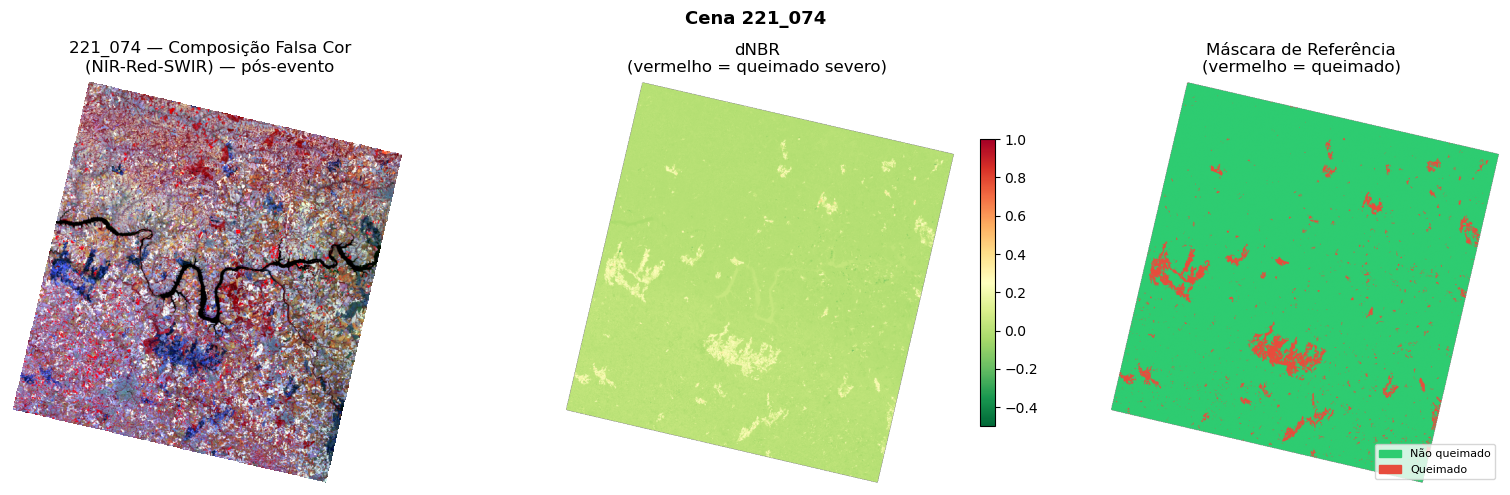
\includegraphics[width=\columnwidth]{figs/rf/fig_cena_221074.png}\\[3pt]
  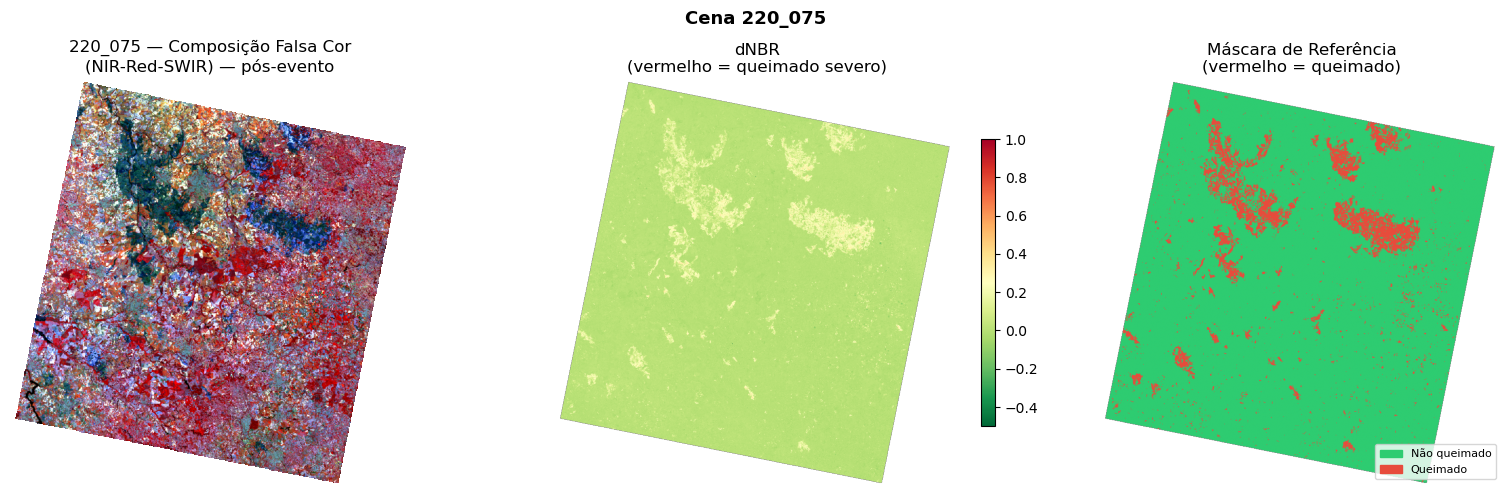
\includegraphics[width=\columnwidth]{figs/rf/fig_cena_220075.png}
  \caption{Composição falsa-cor NIR-Red-SWIR (esq.), dNBR (centro) e
           máscara de referência (dir.) para as cenas 221/074 (cima)
           e 220/075 (baixo). Vermelho indica área queimada.}
  \label{fig:cenas}
\end{figure}

\subsection{Atributos Espectrais}

A Tabela~\ref{tab:features_geral} descreve os atributos espectrais
utilizados pelos modelos supervisionados. Para cada pixel, cinco atributos
são extraídos da imagem pré-queimada e cinco da pós-queimada, formando
um vetor de 10~\textit{features}. A SOM adiciona os índices de variação
temporal $\Delta$NDVI e $\Delta$NBR, totalizando 7~atributos.

\begin{table}[!t]
  \caption{Atributos espectrais utilizados}
  \label{tab:features_geral}
  \centering
  \begin{tabular}{lll}
    \toprule
    \textbf{Atributo} & \textbf{O que mede} & \textbf{Por que importa} \\
    \midrule
    B4 (Red)   & Reflectância no vermelho       & Aumenta após queimada \\
    B5 (NIR)   & Reflectância no IV próximo     & Cai com destruição da vegetação \\
    B7 (SWIR2) & Reflectância no IV onda curta  & Alto em solo exposto/queimado \\
    NDVI       & Índice de vegetação            & Queda indica perda de cobertura \\
    NBR        & Índice de queimada             & Principal discriminador \\
    \bottomrule
  \end{tabular}
\end{table}

\subsection{Desbalanceamento de Classes}

A Tabela~\ref{tab:imbalance_geral} resume a proporção de classes nas três
cenas. O forte desbalanceamento — até 33:1 na cena 222/074 — é o principal
desafio metodológico para todos os modelos supervisionados.

\begin{table}[!t]
  \caption{Proporção de classes por cena}
  \label{tab:imbalance_geral}
  \centering
  \begin{tabular}{lrr}
    \toprule
    \textbf{Cena} & \textbf{\% Queimada} & \textbf{Razão Não-Q:Q} \\
    \midrule
    221/074 & 4,8\%  & 1:19,8 \\
    220/075 & 7,9\%  & 1:11,6 \\
    222/074 & 2,96\% & 1:32,8 \\
    \bottomrule
  \end{tabular}
\end{table}

%=====================================================================
\section{K-Nearest Neighbors (KNN)}

\subsection{Entradas, Saídas e Objetivo}

\textbf{Objetivo:} classificar cada pixel de uma imagem Landsat~8/9 em
\textbf{Classe~0 — Não queimada} ou \textbf{Classe~1 — Queimada} usando o
algoritmo KNN ($K = 5$ vizinhos), com amostras coletadas manualmente via QGIS
e avaliação da generalização espacial em uma cena independente.

O KNN classifica um novo pixel atribuindo a classe majoritária entre seus
$K$ vizinhos mais próximos no espaço de atributos, sem aprender uma
fronteira de decisão explícita durante o treinamento.

\subsection{Metodologia}

\subsubsection{Pré-processamento e Geração das Amostras}

Diferentemente dos demais modelos deste trabalho, as amostras de
treinamento foram coletadas manualmente como pontos vetoriais no QGIS:

\begin{itemize}
  \item \texttt{pontos\_mistos.shp}: amostras das classes~0 e~1;
  \item \texttt{pontos\_nao\_qmd.shp}: amostras exclusivas da classe~0.
\end{itemize}

Os pontos foram convertidos para coordenadas raster e os valores dos
índices espectrais foram extraídos para cada ponto. Pixels em regiões
\textit{NoData} foram removidos. As variáveis foram normalizadas por
\texttt{StandardScaler} antes do treinamento.

\subsubsection{Índices Espectrais Utilizados}

Foram calculados a partir de imagens Landsat pré-fogo (Landsat~8) e
pós-fogo (Landsat~9) os seguintes índices de diferença temporal:

\begin{itemize}
  \item \textbf{dNBR} — \textit{Delta Normalized Burn Ratio};
  \item \textbf{dNBRSWIR} — variante do dNBR com banda SWIR;
  \item \textbf{dNDVI} — \textit{Delta Normalized Difference Vegetation Index}.
\end{itemize}

\subsubsection{Protocolo de Treino e Teste}

O conjunto de dados foi dividido aleatoriamente em 70\% para treinamento
e 30\% para teste interno. Após a validação interna, o modelo foi aplicado
em uma cena Landsat completamente distinta da utilizada no treinamento,
para avaliação de generalização espacial. A Fig.~\ref{fig:knn_cena_treino}
apresenta a cena de treinamento.

\begin{figure}[!t]
  \centering
  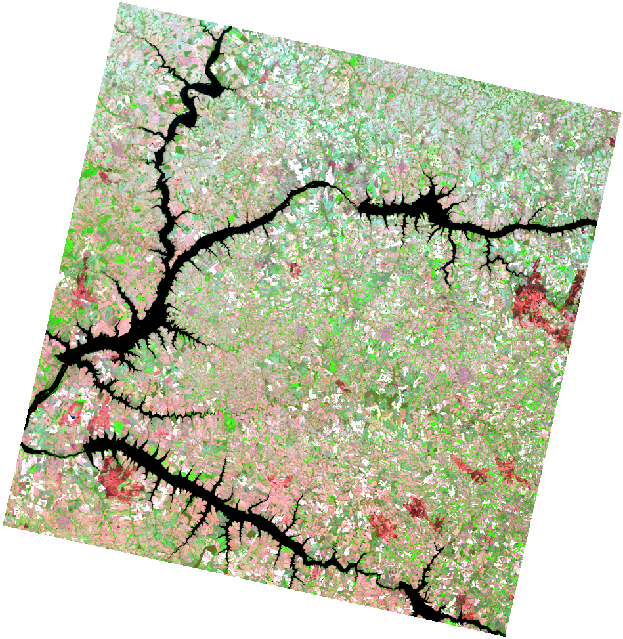
\includegraphics[width=\columnwidth]{imgs_knn/cena_treinamento.png}
  \caption{Cena Landsat utilizada no treinamento do modelo KNN.}
  \label{fig:knn_cena_treino}
\end{figure}

\subsection{Resultados}

\subsubsection{Desempenho no Conjunto Interno (70/30)}

\begin{table}[!t]
  \caption{Métricas no conjunto interno — KNN ($K=5$)}
  \label{tab:knn_train}
  \centering
  \begin{tabular}{lccc}
    \toprule
    \textbf{Classe} & \textbf{Precision} & \textbf{Recall} & \textbf{F1} \\
    \midrule
    0 (Não queimada) & 0,76 & 0,69 & 0,72 \\
    1 (Queimada)     & 0,71 & 0,77 & 0,74 \\
    \midrule
    \multicolumn{3}{l}{\textbf{Accuracy}} & 0,73 \\
    \multicolumn{3}{l}{\textbf{F1 médio}} & 0,73 \\
    \bottomrule
  \end{tabular}
\end{table}

\subsubsection{Generalização em Nova Cena}

O modelo foi avaliado em uma cena Landsat independente. A
Fig.~\ref{fig:knn_cena_teste} apresenta a cena de teste e a classificação
produzida pelo modelo.

\begin{figure}[!t]
  \centering
  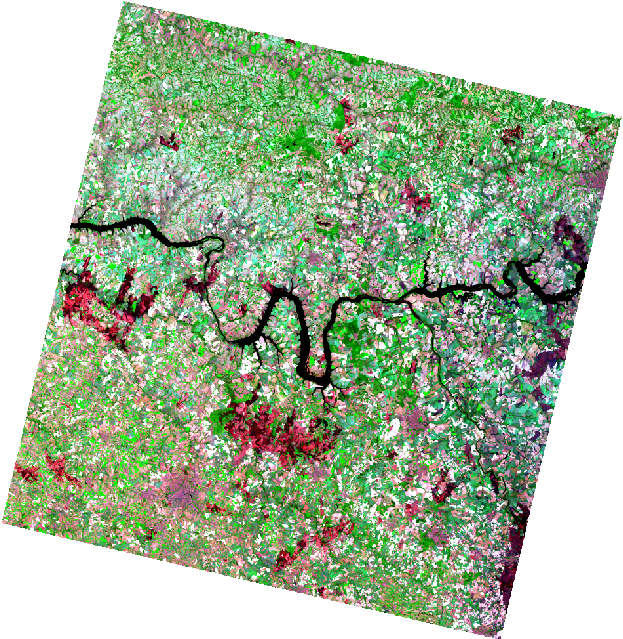
\includegraphics[width=\columnwidth]{imgs_knn/cena_teste.png}
  \caption{Cena Landsat utilizada para teste do modelo KNN.}
  \label{fig:knn_cena_teste}
\end{figure}

\begin{figure}[!t]
  \centering
  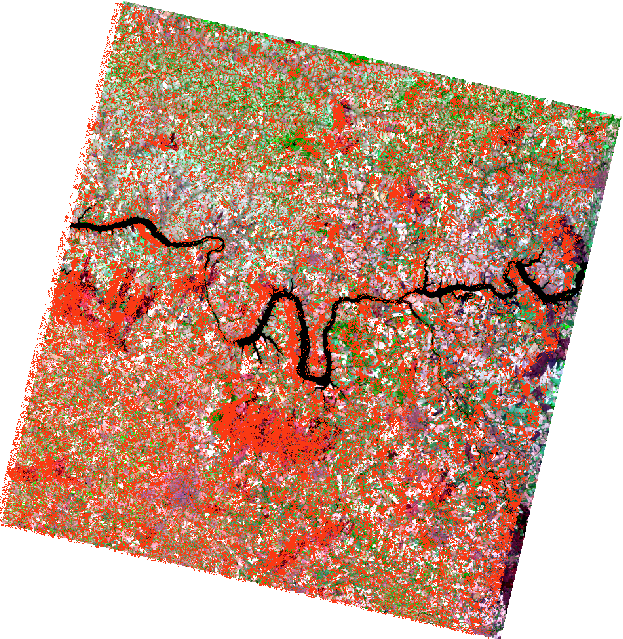
\includegraphics[width=\columnwidth]{imgs_knn/cena_teste_classificada.png}
  \caption{Resultado da classificação do KNN na nova cena. A superestimação
           de área queimada (vermelho) evidencia a elevada taxa de falsos
           positivos.}
  \label{fig:knn_classificada}
\end{figure}

\begin{table}[!t]
  \caption{Métricas na nova cena — KNN ($K=5$)}
  \label{tab:knn_test}
  \centering
  \begin{tabular}{lccc}
    \toprule
    \textbf{Classe} & \textbf{Precision} & \textbf{Recall} & \textbf{F1} \\
    \midrule
    0 (Não queimada) & 0,99 & 0,69 & 0,81 \\
    1 (Queimada)     & 0,09 & 0,82 & 0,17 \\
    \midrule
    \multicolumn{3}{l}{\textbf{Accuracy}} & 0,69 \\
    \multicolumn{3}{l}{\textbf{F1-score (queimada)}} & 0,17 \\
    \bottomrule
  \end{tabular}
\end{table}

A Fig.~\ref{fig:knn_metricas} compara as métricas entre o conjunto interno
e a nova cena, evidenciando a queda de desempenho na generalização.

\begin{figure}[!t]
  \centering
  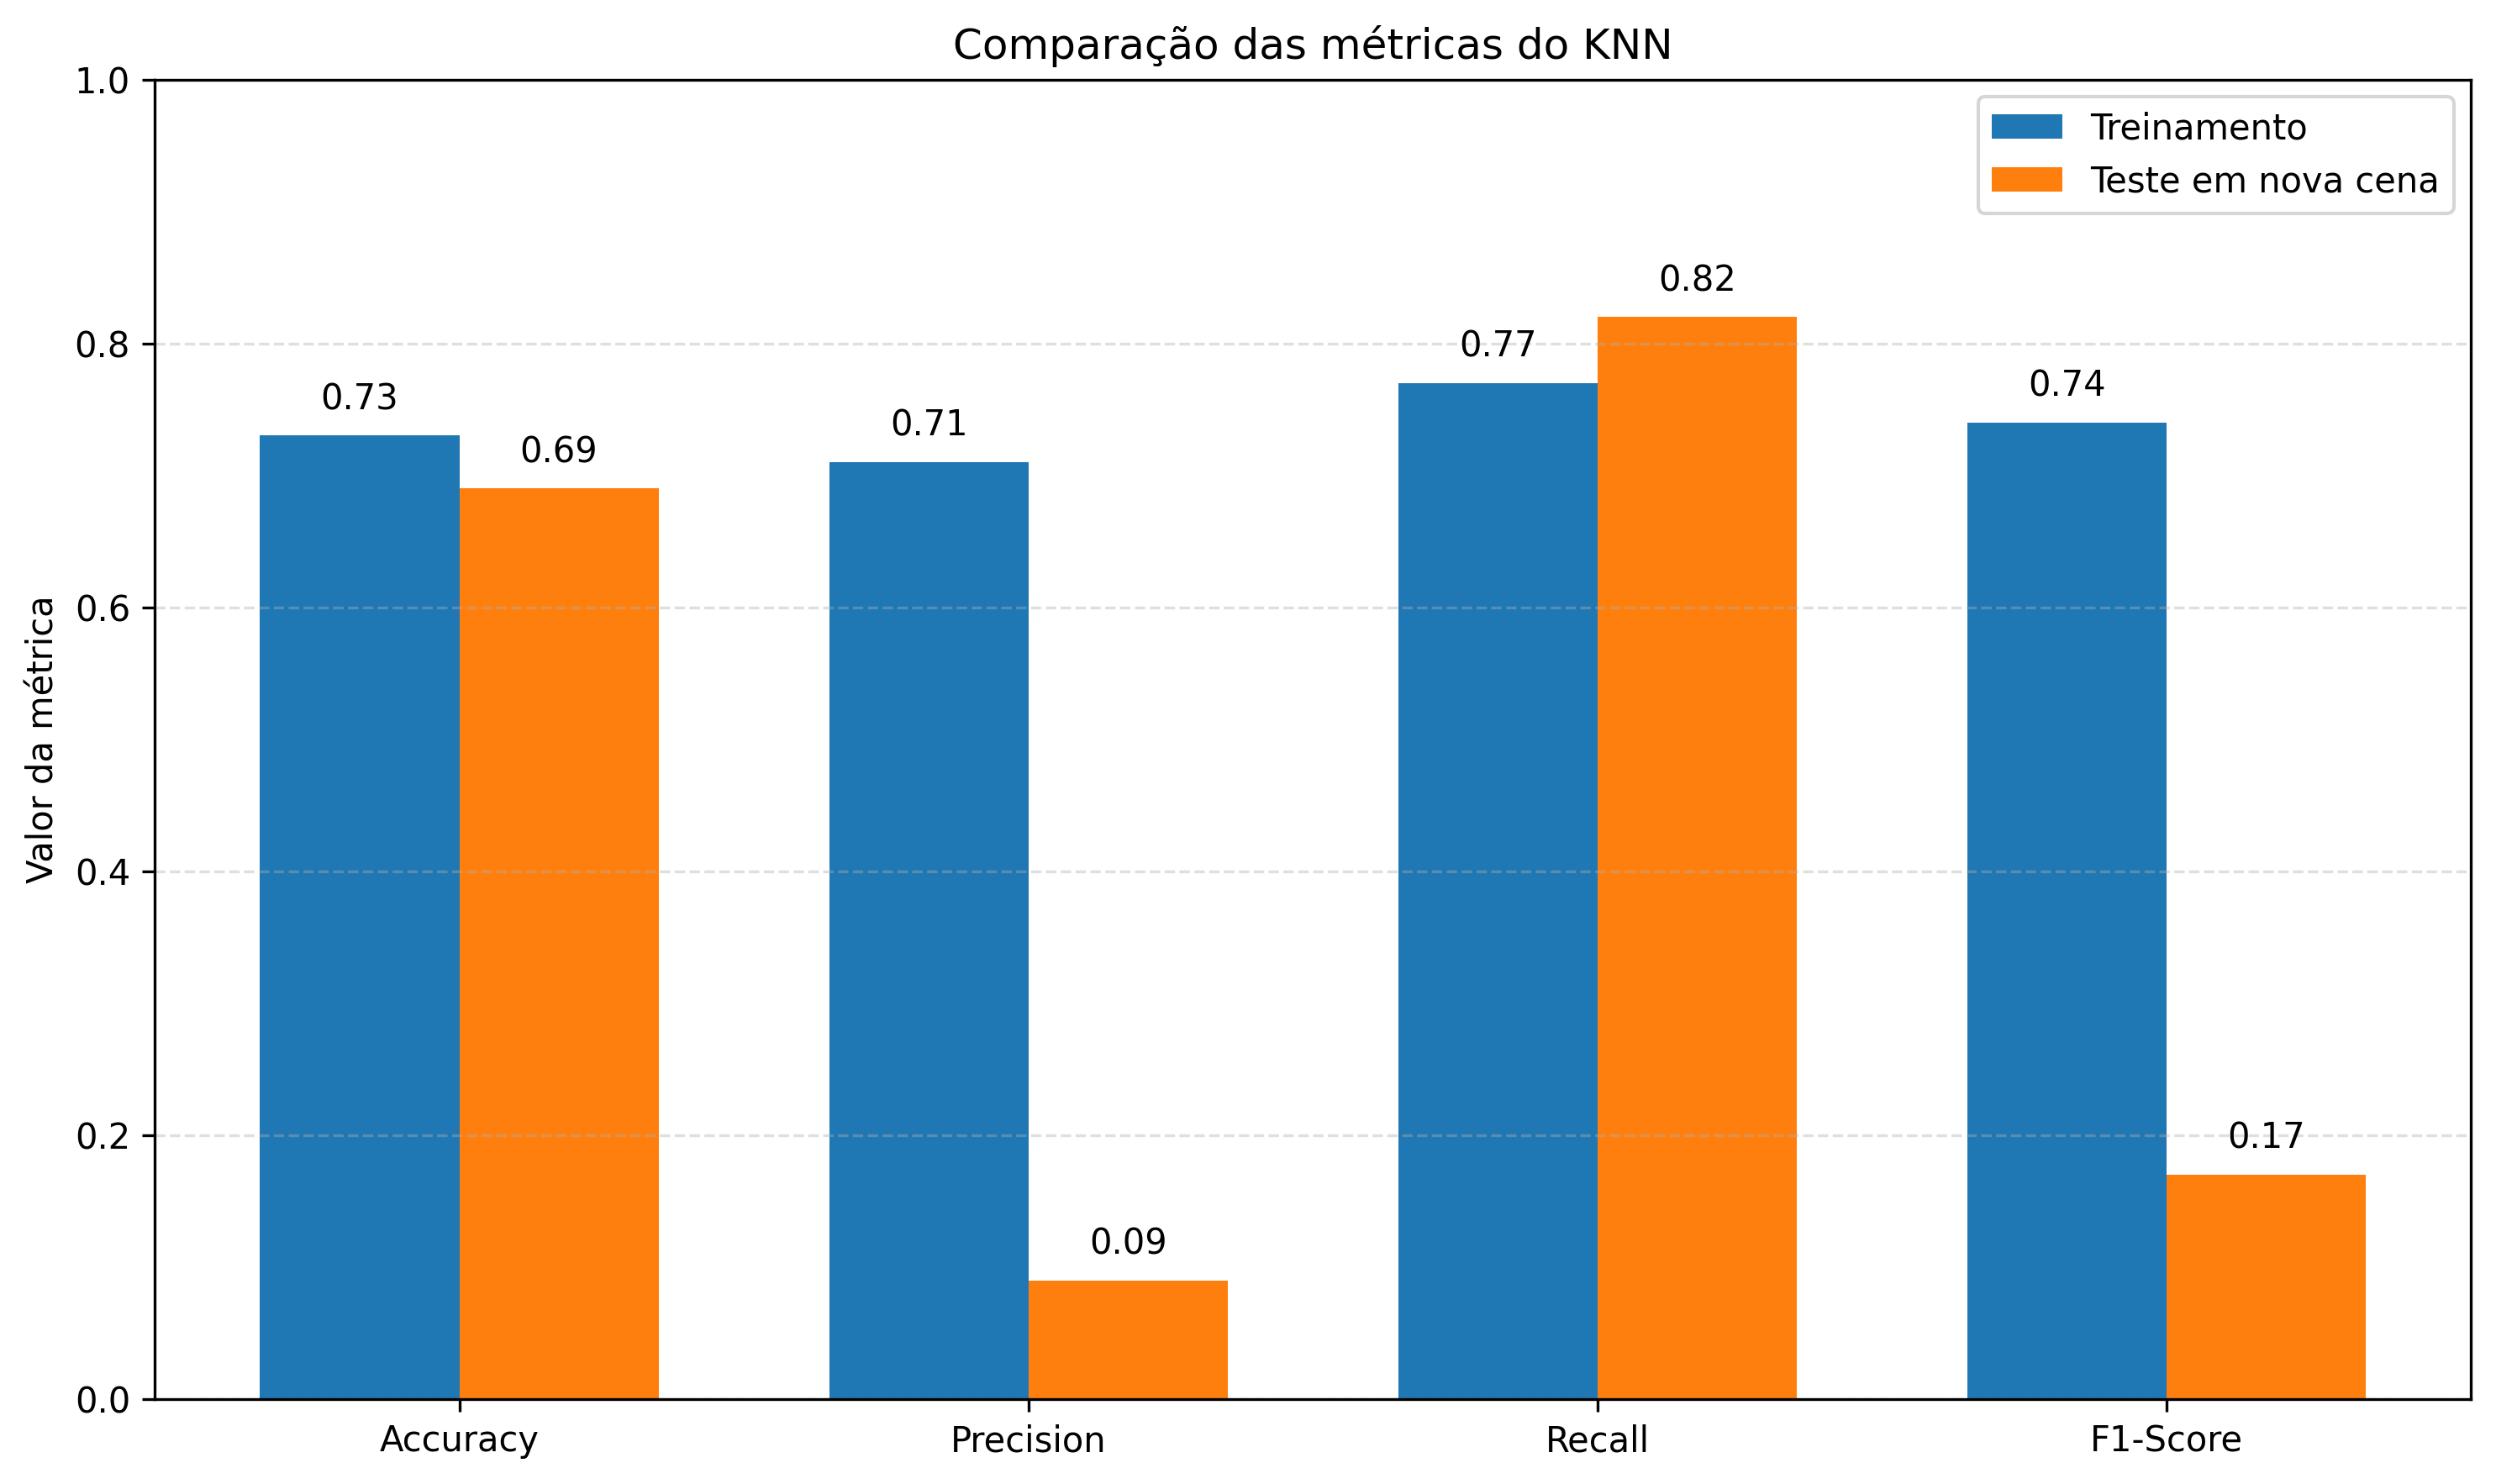
\includegraphics[width=\columnwidth]{imgs_knn/grafico_metricas_knn.png}
  \caption{Comparação das métricas KNN entre treinamento e teste em nova
           cena. A queda na Precision e F1 da classe queimada evidencia
           a limitação de generalização espacial.}
  \label{fig:knn_metricas}
\end{figure}

\subsection{Discussão}

O KNN atingiu 73\% de acurácia no conjunto interno, mas apresentou forte
degradação ao ser aplicado em nova cena: a Precision da classe queimada
caiu para 9\% e o F1 para 0,17, com grande superestimação da área queimada.
As principais causas são: (i)~sensibilidade às diferenças radiométricas
entre cenas; (ii)~dependência das características específicas da cena de
treinamento; e (iii)~uso de índices de diferença temporal (dNBR, dNDVI)
como atributos, que podem introduzir viés dependente da calibração
radiométrica relativa entre datas.

A coleta manual de amostras via QGIS, embora permita maior controle sobre
a qualidade dos pontos, reduz a quantidade de amostras disponíveis e
aumenta o risco de viés de seleção do operador. O KNN também não possui
mecanismo nativo para tratar desbalanceamento de classes, o que contribui
para a elevada taxa de falsos positivos observada.

%=====================================================================
\section{SVM Linear}

\subsection{Entradas, Saídas e Objetivo}

\textbf{Objetivo:} desenvolver um classificador binário baseado em SVM
Linear (\texttt{LinearSVC}) capaz de detectar automaticamente pixels
queimados e não queimados a partir de atributos derivados do índice NDVI
em imagens Landsat~8/9. O modelo é treinado em duas cenas e validado em
uma terceira cena independente.

\begin{table}[!t]
  \caption{Entradas e saídas da SVM Linear}
  \label{tab:svm_linear_io}
  \centering
  \begin{tabular}{ll}
    \toprule
    \textbf{ENTRADA} & \textbf{SAÍDA} \\
    \midrule
    2 atributos por pixel & Predição de classe por pixel \\
    NDVI pré-queimada & 1 = Queimado \\
    NDVI pós-queimada & 0 = Não Queimado \\
    (normalizados) & + relatório de métricas \\
    \bottomrule
  \end{tabular}
\end{table}

\subsection{Metodologia}

\subsubsection{Pré-processamento e Organização dos Dados}

O experimento utilizou imagens Landsat processadas para NDVI em períodos
pré e pós-queimada. Os rasters foram carregados via \texttt{Rasterio} e
ajustados ao menor tamanho comum entre imagens pré e pós-evento. Um
procedimento de limpeza numérica eliminou valores \texttt{NaN}, infinitos
e pixels inválidos. Regiões com corpos d'água foram removidas por máscara
de valores negativos de NDVI, reduzindo falsos positivos causados pela
semelhança espectral com áreas queimadas. Os atributos foram limitados
ao intervalo $[-1, 1]$, garantindo estabilidade numérica.

\subsubsection{Balanceamento e Amostragem}

O forte desbalanceamento entre classes foi tratado por amostragem
balanceada por classe: 25.000~pixels por classe (50.000~amostras totais).
Essa estratégia reduz o viés para a classe dominante, aumenta a
estabilidade estatística e reduz o custo computacional do SVM.

\subsubsection{Treinamento e Validação}

O modelo \texttt{LinearSVC} foi configurado com
\texttt{class\_weight='balanced'} e limite elevado de iterações para
convergência numérica. Os atributos foram normalizados por
\texttt{StandardScaler} (média zero, variância unitária) — etapa
fundamental em modelos SVM, sensíveis à escala. O treinamento utilizou
as cenas 220/075 e 221/074; a cena 222/074 foi reservada exclusivamente
para validação.

\subsection{Resultados}

\subsubsection{Métricas de Desempenho}

\begin{table}[!t]
  \caption{Métricas de desempenho — SVM Linear, cena 222/074}
  \label{tab:svm_linear_metrics}
  \centering
  \begin{tabular}{lc}
    \toprule
    \textbf{Métrica} & \textbf{Valor} \\
    \midrule
    Acurácia (OA)    & 80,14\% \\
    Precision        & 14,04\% \\
    Recall           & 83,43\% \\
    F1-score         & 24,04\% \\
    IoU              & 13,66\% \\
    \bottomrule
  \end{tabular}
\end{table}

O elevado Recall (83,43\%) indica alta capacidade de detecção da classe
queimada. A baixa Precision (14,04\%) evidencia elevada incidência de
falsos positivos — reflexo da limitação de apenas dois atributos de
entrada.

\subsubsection{Matriz de Confusão}

\begin{table}[!t]
  \caption{Matriz de Confusão — SVM Linear, cena 222/074}
  \label{tab:svm_linear_cm}
  \centering
  \begin{tabular}{lcc}
    \toprule
    & \textbf{Pred. Não Queimado} & \textbf{Pred. Queimado} \\
    \midrule
    \textbf{Real Não Queimado} & 38.501 (TN) & 9.616 (FP) \\
    \textbf{Real Queimado}     &    312 (FN) & 1.571 (TP) \\
    \bottomrule
  \end{tabular}
\end{table}

\begin{table}[!t]
  \caption{Classification Report — SVM Linear, cena 222/074}
  \label{tab:svm_linear_report}
  \centering
  \begin{tabular}{lcccc}
    \toprule
    \textbf{Classe} & \textbf{Precision} & \textbf{Recall}
                    & \textbf{F1} & \textbf{Support} \\
    \midrule
    Não queimado (0) & 0,99 & 0,80 & 0,89 & 48.117 \\
    Queimado (1)     & 0,14 & 0,83 & 0,24 & 1.883  \\
    \midrule
    Accuracy         & \multicolumn{4}{c}{0,80 (50.000 amostras)} \\
    Macro avg        & 0,57 & 0,82 & 0,56 & 50.000 \\
    Weighted avg     & 0,96 & 0,80 & 0,86 & 50.000 \\
    \bottomrule
  \end{tabular}
\end{table}

\begin{figure}[!t]
  \centering
  
\includegraphics[width=0.85\columnwidth]{figs/svm_linear/fig_cm.png}
  \caption{Matriz de Confusão — SVM Linear, cena~222/074.
           TN=38.501, FP=9.616, FN=312, TP=1.571.}
  \label{fig:svm_linear_cm}
\end{figure}

\subsection{Discussão}

Os resultados confirmam que o SVM Linear generaliza a detecção de áreas
queimadas entre cenas Landsat com alta sensibilidade (Recall~$= 83\%$).
A principal limitação reside na restrição a apenas dois atributos de
entrada: solos expostos e áreas queimadas apresentam valores de NDVI
similares, causando elevada taxa de falsos positivos. A incorporação de
atributos adicionais — bandas B4, B5, B7 e o NBR multitemporal — seria
a principal via de melhoria.

%=====================================================================
\section{SVM com Kernel RBF}

\subsection{Entradas, Saídas e Objetivo}

\textbf{Objetivo:} dado um pixel de uma imagem de satélite, determinar se
ele pertence a uma área que sofreu queimada recente — classificação binária
supervisionada pixel a pixel, com generalização para cenas geograficamente
independentes.

\begin{table}[!t]
  \caption{Entradas e saídas da SVM RBF}
  \label{tab:svm_rbf_io}
  \centering
  \begin{tabular}{ll}
    \toprule
    \textbf{ENTRADA} & \textbf{SAÍDA} \\
    \midrule
    10 atributos por pixel & Classe por pixel \\
    Bandas B4, B5, B7 & 1 = Queimado \\
    Índices NDVI e NBR & 0 = Não Queimado \\
    (pré e pós-queimada) & + mapa de probabilidade \\
    \bottomrule
  \end{tabular}
\end{table}

\subsection{Metodologia}

\subsubsection{Dados e Estratégia de Treino/Teste}

Foram usadas três cenas Landsat~8/9 localizadas no estado de São Paulo
(agosto de 2024):

\begin{itemize}
  \item \textbf{220/075} — cena de \textbf{treino e validação}, com máscara
        de referência disponível;
  \item \textbf{221/074} e \textbf{222/074} — cenas de \textbf{teste cego},
        geograficamente distintas, nunca vistas pelo modelo durante o treino.
\end{itemize}

Imagens com cobertura de nuvens foram incluídas como amostras da classe
não queimada, aumentando a robustez do modelo a condições de nebulosidade.

\subsubsection{Como a SVM RBF Funciona}

\begin{enumerate}
  \item \textbf{Treinamento}: a SVM aprende uma fronteira de decisão
        não-linear no espaço dos 10~atributos. Apenas os vetores de suporte
        — amostras mais próximas da fronteira — definem o modelo final.
  \item \textbf{Otimização}: os hiperparâmetros $C$ e $\gamma$ foram
        ajustados via \textbf{Optuna} (50~tentativas, TPE Sampler),
        maximizando o $F_1$ em validação cruzada.
  \item \textbf{Inferência}: classificação em lotes sobre a cena completa,
        produzindo a classe binária e a probabilidade de cada pixel.
\end{enumerate}

Na composição falsa-cor B7/B5/B4, áreas queimadas aparecem em vermelho
intenso — reflexo da alta reflectância em SWIR2 e colapso do NIR,
como ilustra a Fig.~\ref{fig:svm_rbf_falsa_cor}.

\begin{figure}[!t]
  \centering
  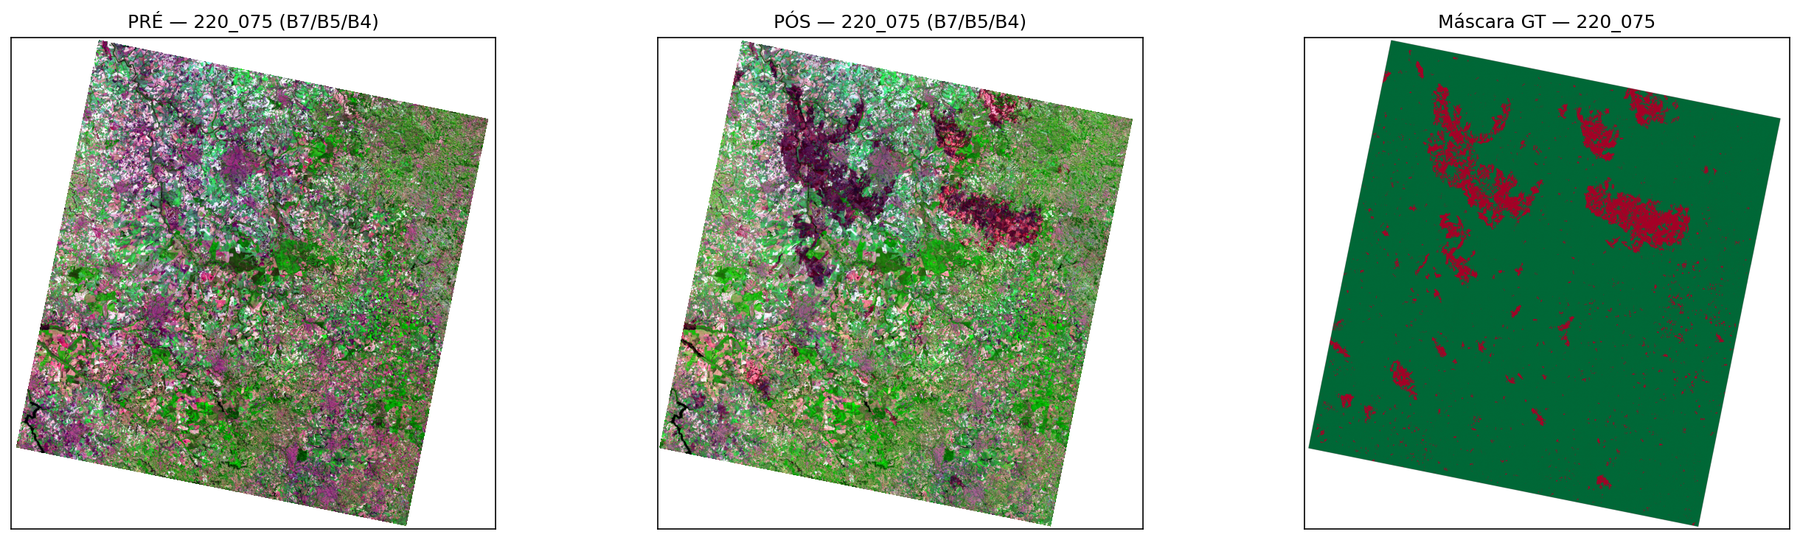
\includegraphics[width=\columnwidth]{figs/svm_rbf/fig_falsa_cor.png}
  \caption{Cena de treino 220/075: composição falsa-cor pré-queimada (esq.),
           pós-queimada (centro) e máscara \textit{ground-truth} (dir.).
           Áreas queimadas em vermelho na imagem pós-queimada.}
  \label{fig:svm_rbf_falsa_cor}
\end{figure}

\subsection{Resultados}

\subsubsection{Otimização de Hiperparâmetros}

A busca pelo Optuna concentrou os melhores resultados em valores altos de
regularização ($C$), indicando fronteira de decisão complexa que se
beneficia de menor penalização da margem. A Fig.~\ref{fig:svm_rbf_optuna}
mostra a convergência do $F_1$.

\begin{figure}[!t]
  \centering
  
\includegraphics[width=\columnwidth]{figs/svm_rbf/fig_optuna.png}
  \caption{Busca de hiperparâmetros SVM RBF — Optuna (50~tentativas):
           evolução do melhor $F_1$ acumulado (esq.) e distribuição dos
           pontos testados no espaço $C \times \gamma$ (dir.),
           coloridos pelo $F_1$ obtido.}
  \label{fig:svm_rbf_optuna}
\end{figure}

\subsubsection{Desempenho nos Conjuntos de Teste}

\begin{table}[!t]
  \caption{Desempenho da SVM RBF em todos os conjuntos}
  \label{tab:svm_rbf_results}
  \centering
  \setlength{\tabcolsep}{4pt}
  \begin{tabular}{lcccc}
    \toprule
    \textbf{Conjunto} & \textbf{Acurácia} & \textbf{Precisão}
                      & \textbf{Recall} & \textbf{F1} \\
    \midrule
    Treino (50k amostras)     & 99,96\% & 98,69\% & 100,00\% & \textbf{99,34\%} \\
    Validação (12M pixels)    & 99,85\% & 98,40\% &  99,76\% & \textbf{99,07\%} \\
    Teste cego 221/074 (40M)  & 99,91\% & 98,60\% &  99,64\% & \textbf{99,12\%} \\
    Teste cego 222/074 (40M)  & 99,88\% & 96,83\% &  99,30\% & \textbf{98,05\%} \\
    \bottomrule
    \multicolumn{5}{l}{AUC-ROC $= 1{,}000$ em todos os conjuntos.}
  \end{tabular}
\end{table}

\subsubsection{Matrizes de Confusão}

\begin{table}[!t]
  \caption{Matriz de Confusão — Teste Cego 221/074}
  \label{tab:svm_rbf_cm221}
  \centering
  \begin{tabular}{lcc}
    \toprule
    & \textbf{Pred.\ Não Queimado} & \textbf{Pred.\ Queimado} \\
    \midrule
    \textbf{Real Não Queimado} & 38.143.005 (TN) & 27.725 (FP) \\
    \textbf{Real Queimado}     &      2.669 (FN) & 720.603 (TP) \\
    \bottomrule
  \end{tabular}
\end{table}

\begin{table}[!t]
  \caption{Matriz de Confusão — Teste Cego 222/074}
  \label{tab:svm_rbf_cm222}
  \centering
  \begin{tabular}{lcc}
    \toprule
    & \textbf{Pred.\ Não Queimado} & \textbf{Pred.\ Queimado} \\
    \midrule
    \textbf{Real Não Queimado} & 38.853 (TN)     & 8.177 (FP)      \\
    \textbf{Real Queimado}     &  8.571 (FN)     & 1.180.989 (TP)  \\
    \bottomrule
  \end{tabular}
\end{table}

\begin{figure}[!t]
  \centering
  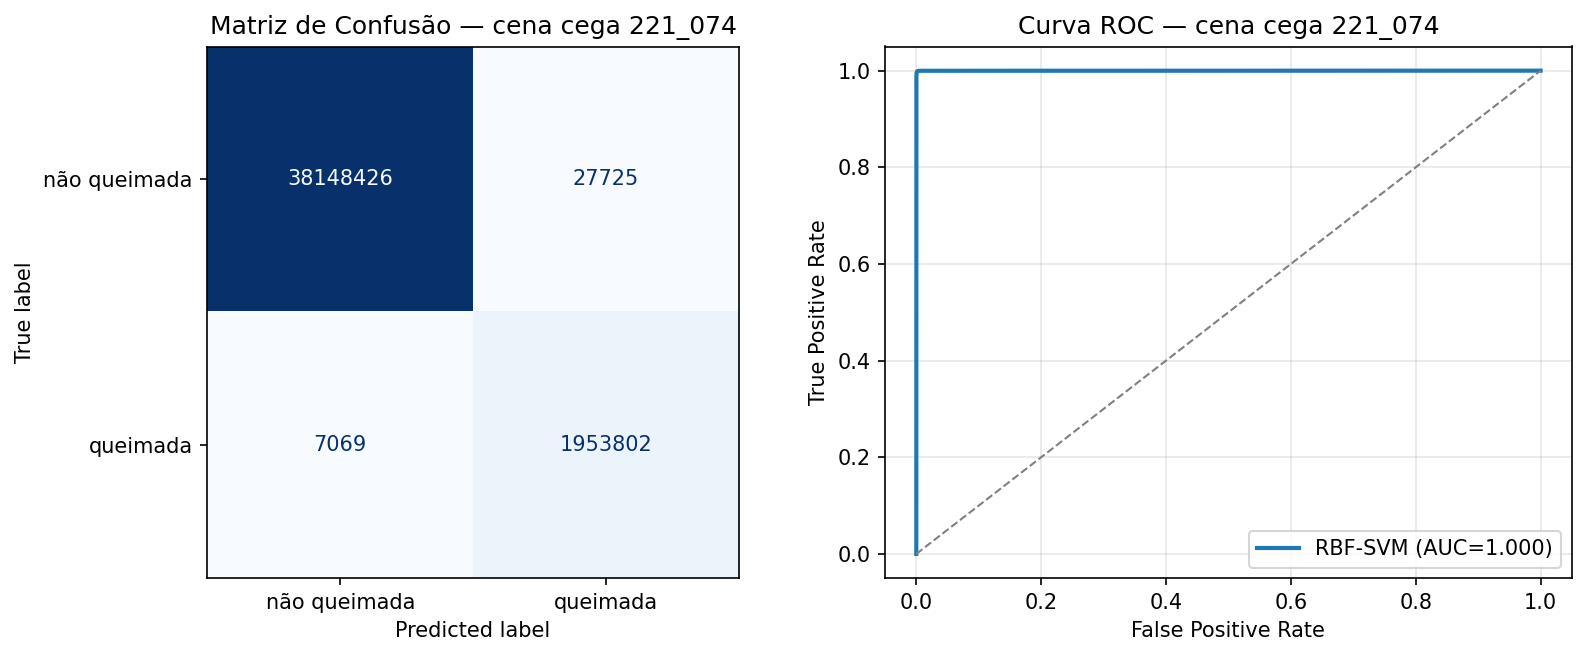
\includegraphics[width=\columnwidth]{figs/svm_rbf/fig_cm_221.png}\\[4pt]
  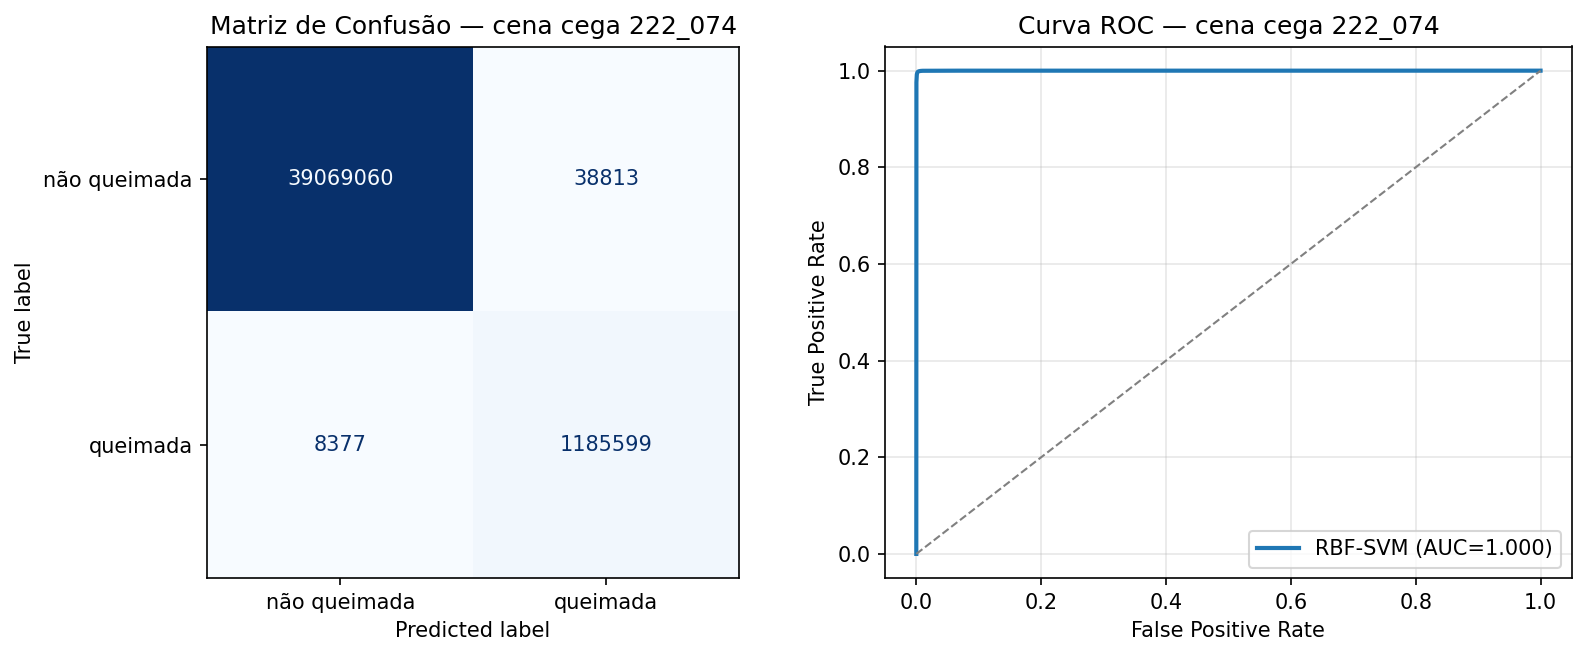
\includegraphics[width=\columnwidth]{figs/svm_rbf/fig_cm_222.png}
  \caption{Matrizes de confusão e curvas ROC da SVM RBF:
           cena~221/074 — F1=99,1\% (cima) e cena~222/074 — F1=98,1\% (baixo).
           AUC-ROC=1,000 em ambas.}
  \label{fig:svm_rbf_cm_roc}
\end{figure}

\subsubsection{Vetores de Suporte}

O modelo utilizou apenas \textbf{105 vetores de suporte} sobre 50~mil
amostras de treino. Esse número reduzido confirma que as classes são
espectralmente bem separadas: a fronteira de decisão pode ser definida
com um conjunto mínimo de exemplos representativos.

\subsection{Discussão}

Os resultados ($F_1 > 98\%$, AUC~$= 1{,}000$) demonstram que a SVM~RBF
aprendeu a identificar áreas queimadas a partir de amostras de uma única
cena e generalizou para regiões geograficamente distintas. A estabilidade
entre os dois testes cegos ($F_1 = 99{,}12\%$ e $98{,}05\%$) evidencia
robustez da assinatura espectral aprendida. A capacidade de aprender
fronteiras não-lineares distingue a SVM~RBF da versão linear, capturando
relações não-lineares entre as 10~features multitemporais que são
determinantes para separar cicatrizes de solos expostos e sombras.

%=====================================================================
\section{Multilayer Perceptron (MLP)}

\subsection{Entradas, Saídas e Objetivo}

\textbf{Objetivo:} classificar cada pixel de uma imagem Landsat~8/9 em
\textbf{Classe~0 — Não queimada} ou \textbf{Classe~1 — Queimada}, usando
rede neural treinada em múltiplas cenas e avaliada de forma cega.

\begin{table}[!t]
  \caption{Entradas e saídas da MLP}
  \label{tab:mlp_io}
  \centering
  \begin{tabular}{ll}
    \toprule
    \textbf{ENTRADA} & \textbf{SAÍDA} \\
    \midrule
    10 valores por pixel & Probabilidade de cada classe \\
    Pré-queimada: B4, B5, B7, NDVI, NBR & $\hat{p}(\text{queimada})$ \\
    Pós-queimada: B4, B5, B7, NDVI, NBR & $\hat{p}(\text{não queimada})$ \\
    (normalizados por \texttt{StandardScaler}) & (via Softmax + limiar 0,5) \\
    \bottomrule
  \end{tabular}
\end{table}

\subsection{Metodologia}

\subsubsection{Dados, Protocolo e Desbalanceamento}

Três cenas Landsat~8/9 foram utilizadas:

\begin{itemize}
  \item \textbf{220/075} (LC09, 29/08): treino e validação;
  \item \textbf{221/074} (LC08, 28/08): treino e validação;
  \item \textbf{222/074} (LC09, 27/08): teste cego.
\end{itemize}

\textbf{Protocolo:}
\begin{itemize}
  \item \textbf{Treino + Validação}: 100k~pixels/classe de cada cena
        $= 400$k~pixels totais (balanceados 50/50).
  \item \textbf{Validação}: Stratified 5-Fold CV no conjunto de treino.
  \item \textbf{Teste cego}: todos os 40,3~M~pixels válidos da cena
        222/074 (2,96\% queimada).
\end{itemize}

O dataset completo apresenta razão de até 18:1 entre classes.
A Fig.~\ref{fig:mlp_dist} ilustra a distribuição.

\begin{figure}[!t]
  \centering
  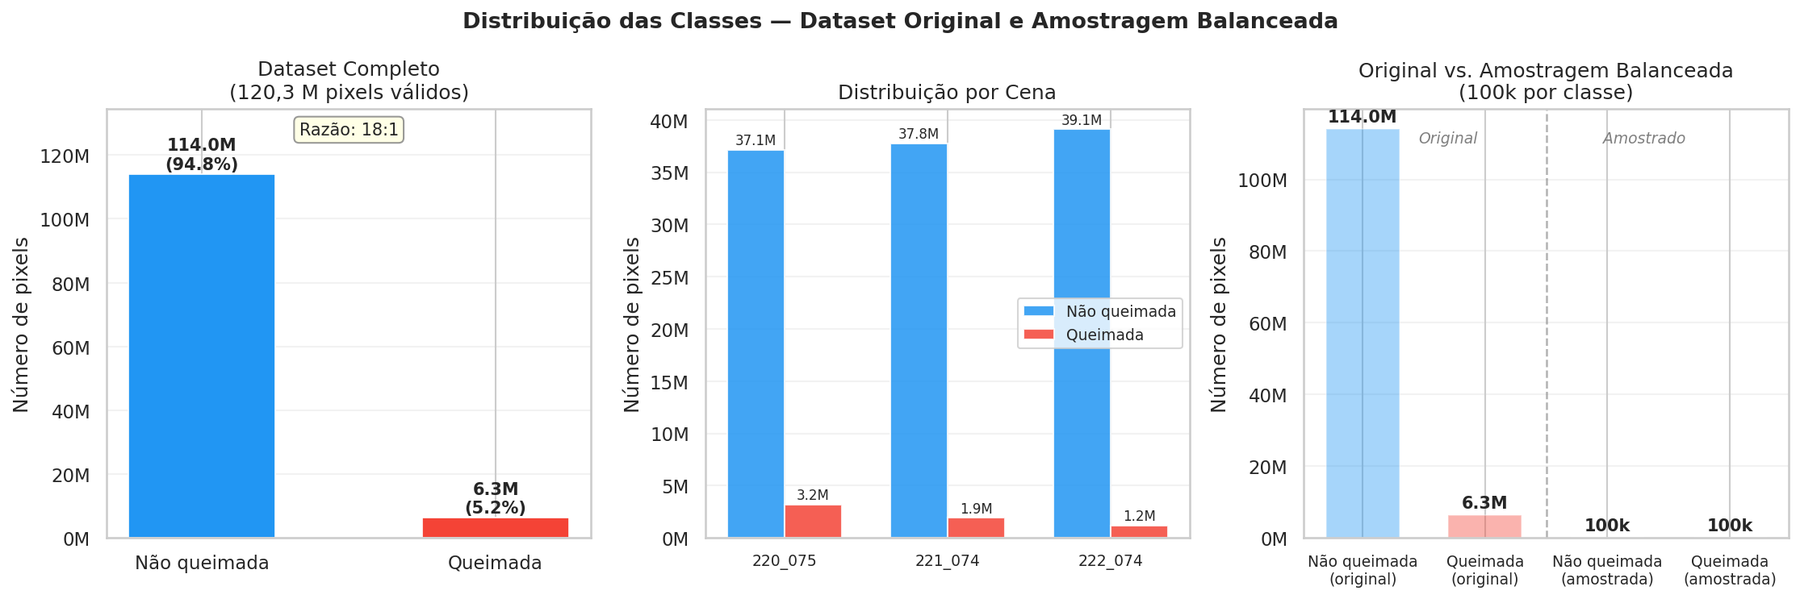
\includegraphics[width=\columnwidth]{figs/mlp/fig_distribuicao.png}
  \caption{Distribuição das classes: dataset completo (esq.), por cena
           (centro) e amostragem balanceada 100k/classe (dir.).
           Razão original 18:1.}
  \label{fig:mlp_dist}
\end{figure}

\subsubsection{Arquitetura e Treinamento}

\begin{table}[!t]
  \caption{Arquitetura da MLP}
  \label{tab:mlp_arch}
  \centering
  \begin{tabular}{ll}
    \toprule
    \textbf{Componente} & \textbf{Especificação} \\
    \midrule
    Entrada        & 10 neurônios (B4, B5, B7, NDVI, NBR $\times$ pré+pós) \\
    Camadas ocultas & $2 \times 64$ — BatchNorm1d + ReLU + Dropout(0,256) \\
    Saída          & 2 logits $\rightarrow$ CrossEntropyLoss com pesos \\
    Anti-leakage   & StandardScaler fitado somente nos dados de treino \\
    Regularização  & Early Stopping (paciência~10); Dropout estocástico \\
    \bottomrule
  \end{tabular}
\end{table}

A otimização de hiperparâmetros foi realizada com \textbf{Optuna TPE
Sampler} (5~\textit{trials}, \texttt{MedianPruner}), minimizando a
\textit{val\_loss}. Parâmetros fixos: Adam ($\alpha = 10^{-3}$),
batch~1024, $n_\text{epochs} \leq 50$.

\subsection{Resultados}

\subsubsection{Validação Cruzada — Métricas por Fold}

\begin{table}[!t]
  \caption{Stratified 5-Fold CV — Cenas 220/075 + 221/074 (400k pixels)}
  \label{tab:mlp_cv}
  \centering
  \begin{tabular}{cccccc}
    \toprule
    \textbf{Fold} & \textbf{Acc.} & \textbf{Prec.} & \textbf{Recall}
                  & \textbf{F1} & \textbf{AUC-ROC} \\
    \midrule
    1 & 0,7309 & 0,7454 & 0,7013 & 0,7227 & 0,8099 \\
    2 & 0,7317 & 0,7564 & 0,6835 & 0,7181 & 0,8114 \\
    3 & 0,7321 & 0,7472 & 0,7017 & 0,7237 & 0,8108 \\
    4 & 0,7345 & 0,7586 & 0,6880 & 0,7216 & 0,8143 \\
    5 & 0,7342 & 0,7563 & 0,6912 & 0,7223 & 0,8135 \\
    \midrule
    \textbf{Média} & \textbf{0,7327} & \textbf{0,7528} & \textbf{0,6931}
                   & \textbf{0,7217} & \textbf{0,8120} \\
    \textbf{DP}    & 0,0015 & 0,0055 & 0,0079 & 0,0022 & 0,0019 \\
    \bottomrule
  \end{tabular}
\end{table}

O baixo desvio padrão entre folds indica estabilidade e ausência de
overfitting. A Fig.~\ref{fig:mlp_curvas} mostra as métricas por fold
e a curva de \textit{loss} média.

\begin{figure}[!t]
  \centering
  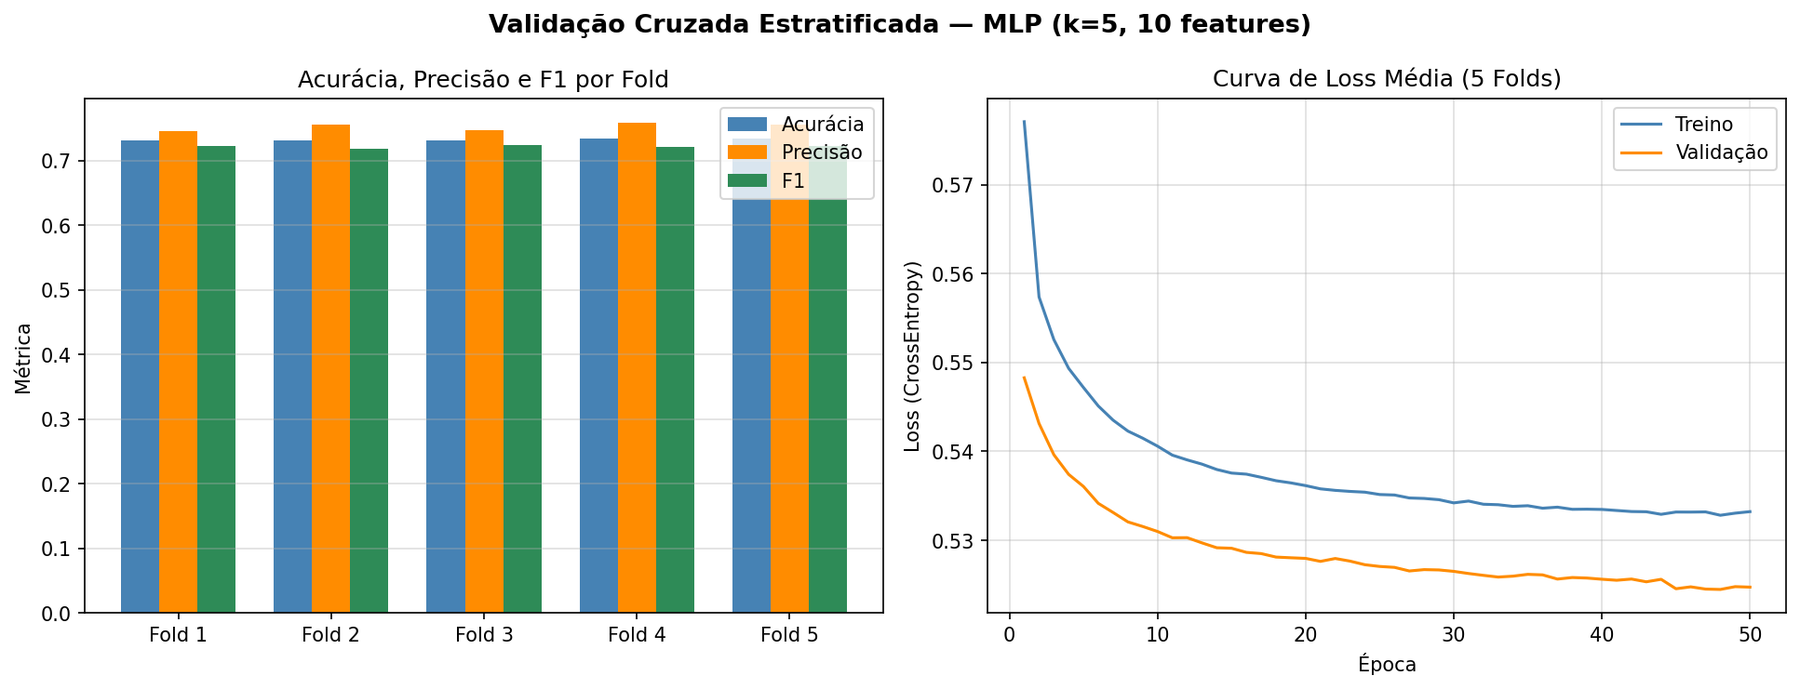
\includegraphics[width=\columnwidth]{figs/mlp/fig_curvas_val.png}
  \caption{Validação cruzada estratificada ($k=5$, 10~features):
           accuracy, precision e F1 por fold (esq.) e curva de
           \textit{loss} média (dir.).}
  \label{fig:mlp_curvas}
\end{figure}

\subsubsection{Teste Cego — Cena 222/074}

\begin{table}[!t]
  \caption{Comparação validação cruzada vs.\ teste cego — MLP}
  \label{tab:mlp_test}
  \centering
  \setlength{\tabcolsep}{4pt}
  \begin{tabular}{lccccc}
    \toprule
    \textbf{Conjunto} & \textbf{Acc.} & \textbf{Prec.}
                      & \textbf{Recall} & \textbf{F1} & \textbf{AUC} \\
    \midrule
    Val.\ cruzada (média)   & 0,733 & 0,753 & 0,693 & 0,722 & 0,812 \\
    Teste 222/074 (40M)     & 0,830 & 0,116 & 0,713 & 0,199$^{*}$ & 0,830 \\
    \bottomrule
    \multicolumn{6}{l}{$^{*}$Precision baixa. AUC indica separabilidade real.}
  \end{tabular}
\end{table}

\begin{table}[!t]
  \caption{Matriz de Confusão — MLP, cena 222/074 (Teste Cego)}
  \label{tab:mlp_cm}
  \centering
  \begin{tabular}{lcc}
    \toprule
    & \textbf{Pred.\ Não Queimada} & \textbf{Pred.\ Queimada} \\
    \midrule
    \textbf{Real Não Queimada} & 32.615.748 (TN) & 6.492.125 (FP) \\
    \textbf{Real Queimada}     &    342.867 (FN) &   851.109 (TP) \\
    \bottomrule
  \end{tabular}
\end{table}

\begin{figure}[!t]
  \centering
  \begin{minipage}[b]{0.48\columnwidth}
    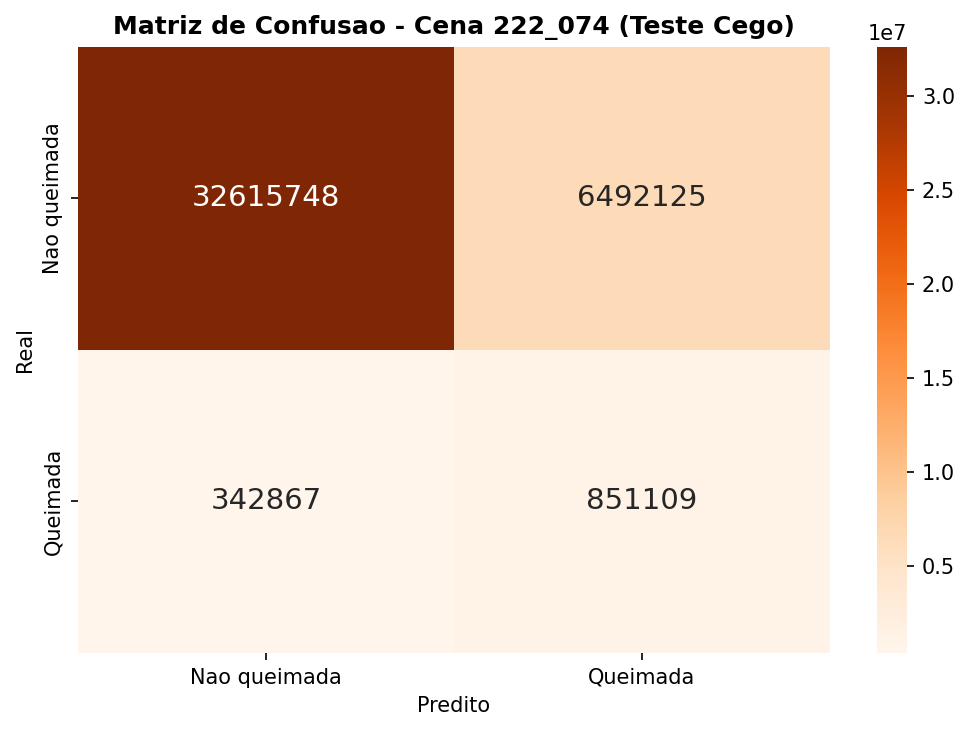
\includegraphics[width=\textwidth]{figs/mlp/fig_cm.png}
    \caption*{(a) Matriz de Confusão}
  \end{minipage}
  \hfill
  \begin{minipage}[b]{0.48\columnwidth}
    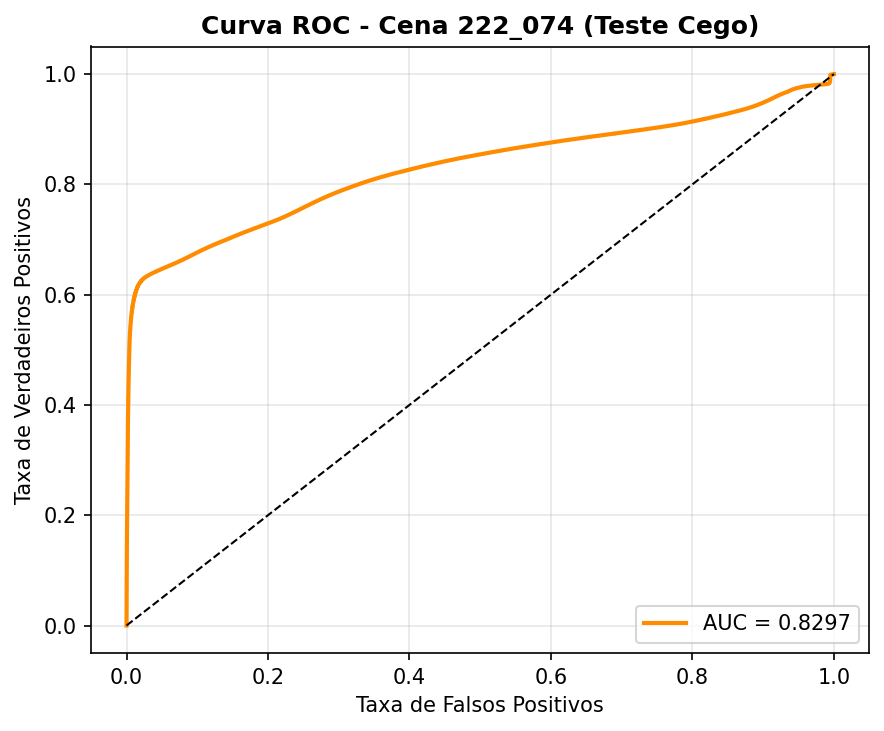
\includegraphics[width=\textwidth]{figs/mlp/fig_roc.png}
    \caption*{(b) Curva ROC}
  \end{minipage}
  \caption{Teste cego 222/074: (a) CM e (b) Curva ROC — AUC=0,830.}
  \label{fig:mlp_cm_roc}
\end{figure}

\subsection{Discussão}

A diferença entre validação cruzada ($F_1 = 0{,}722$) e teste cego
($F_1 = 0{,}199$) é esperada: o treino usou distribuição 50/50, enquanto a
cena de teste possui apenas 2,96\% de queimados. O AUC~$= 0{,}830$ no
teste confirma boa discriminação no espaço de probabilidade — a queda no
$F_1$ é consequência do desbalanceamento e do limiar fixo em 0,5.
Ajuste de threshold via curva Precision-Recall equilibraria melhor as
métricas. A confusão entre solos expostos e cicatrizes recentes é a
principal limitação, compartilhada com todos os métodos que utilizam
apenas assinatura espectral sem índice de diferença.

%=====================================================================
\section{Self-Organizing Map (SOM)}

\subsection{Entradas, Saídas e Objetivo}

\textbf{Objetivo:} identificar automaticamente áreas queimadas em imagens
de satélite, classificando cada pixel em \textbf{Queimada},
\textbf{Não Queimada} ou \textbf{Água} — \textbf{sem nenhuma amostra
rotulada}.

\begin{table}[!t]
  \caption{Entradas e saídas da SOM}
  \label{tab:som_io}
  \centering
  \begin{tabular}{ll}
    \toprule
    \textbf{ENTRADA} & \textbf{SAÍDA} \\
    \midrule
    7 atributos por pixel     & Classe por pixel \\
    Bandas B4, B5, B7         & Queimada \\
    Índices NDVI e NBR        & Não Queimada \\
    Variação $\Delta$NDVI e $\Delta$NBR & Água \\
    (pré e pós-queimada)      & (mapa georreferenciado) \\
    \bottomrule
  \end{tabular}
\end{table}

\subsection{Metodologia}

\subsubsection{Dados}

A cena utilizada é Landsat~8 (30~m, agosto de 2024) do Cerrado
brasileiro, cena~221/074, com par pré e pós-queimada. Os atributos são
normalizados antes do treinamento. Os índices $\Delta$NBR e $\Delta$NDVI
são os mais informativos para identificar cicatrizes de fogo.
A Fig.~\ref{fig:som_bandas} ilustra todos os atributos de entrada.

\begin{figure}[!t]
  \centering
  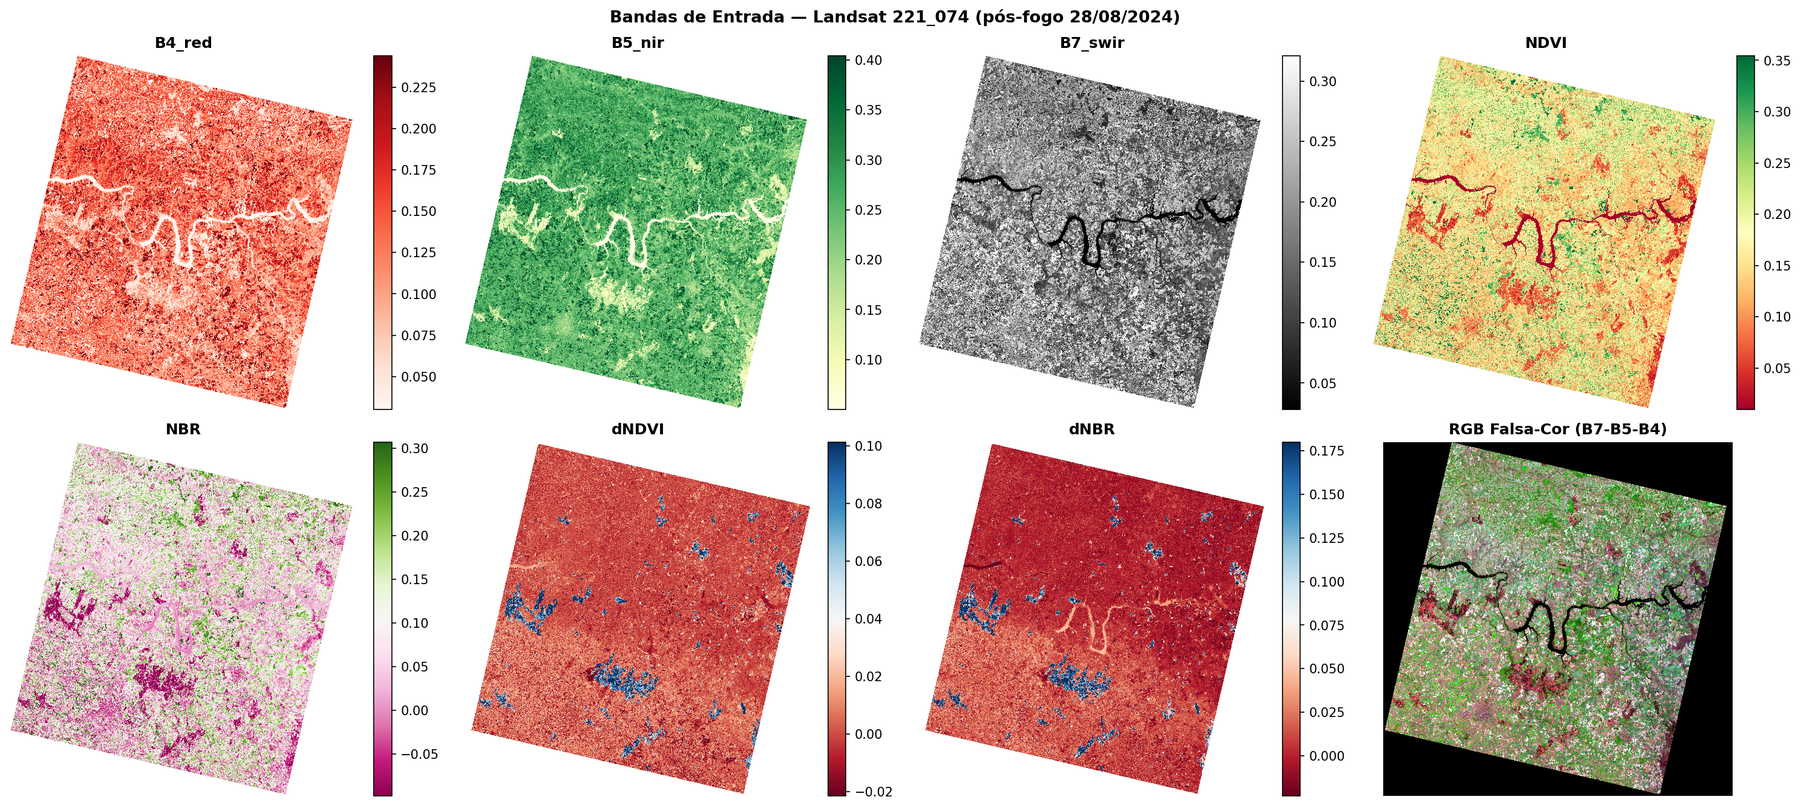
\includegraphics[width=\columnwidth]{figs/som/fig_bandas.png}
  \caption{Atributos de entrada — SOM, cena 221/074 (28/08/2024).
           Os índices $\Delta$NBR e $\Delta$NDVI (última linha) revelam
           com nitidez as cicatrizes de queimada.}
  \label{fig:som_bandas}
\end{figure}

\subsubsection{Como a SOM Funciona}

\begin{enumerate}
  \item \textbf{Treinamento}: organiza neurônios em uma grade~2D de forma
        que pixels espectralmente similares ativem neurônios próximos.
  \item \textbf{Agrupamento}: os pesos dos neurônios são agrupados em
        3~clusters por K-Means.
  \item \textbf{Atribuição}: cada cluster recebe rótulo semântico por
        heurística espectral — sem rótulos humanos: $\Delta$NBR alto
        $\to$ Queimada; NIR baixo + NDVI negativo $\to$ Água;
        demais $\to$ Não Queimada.
  \item \textbf{Inferência}: cada pixel é classificado pela classe do
        neurônio mais próximo (BMU — \textit{Best Matching Unit}).
\end{enumerate}

\subsubsection{Otimização de Hiperparâmetros com Optuna}

Os hiperparâmetros da grade foram otimizados por \textbf{Optuna}
(20~tentativas, TPE Sampler). A configuração ótima utiliza grade
$15\times15$~neurônios. A função de avaliação combina Quantization Error
e Topographic Error:

\begin{equation}
  \mathrm{Score} = 0{,}7 \cdot \mathrm{QE} + 0{,}3 \cdot \mathrm{TE}
  \label{eq:som_score}
\end{equation}

\begin{figure}[!t]
  \centering
  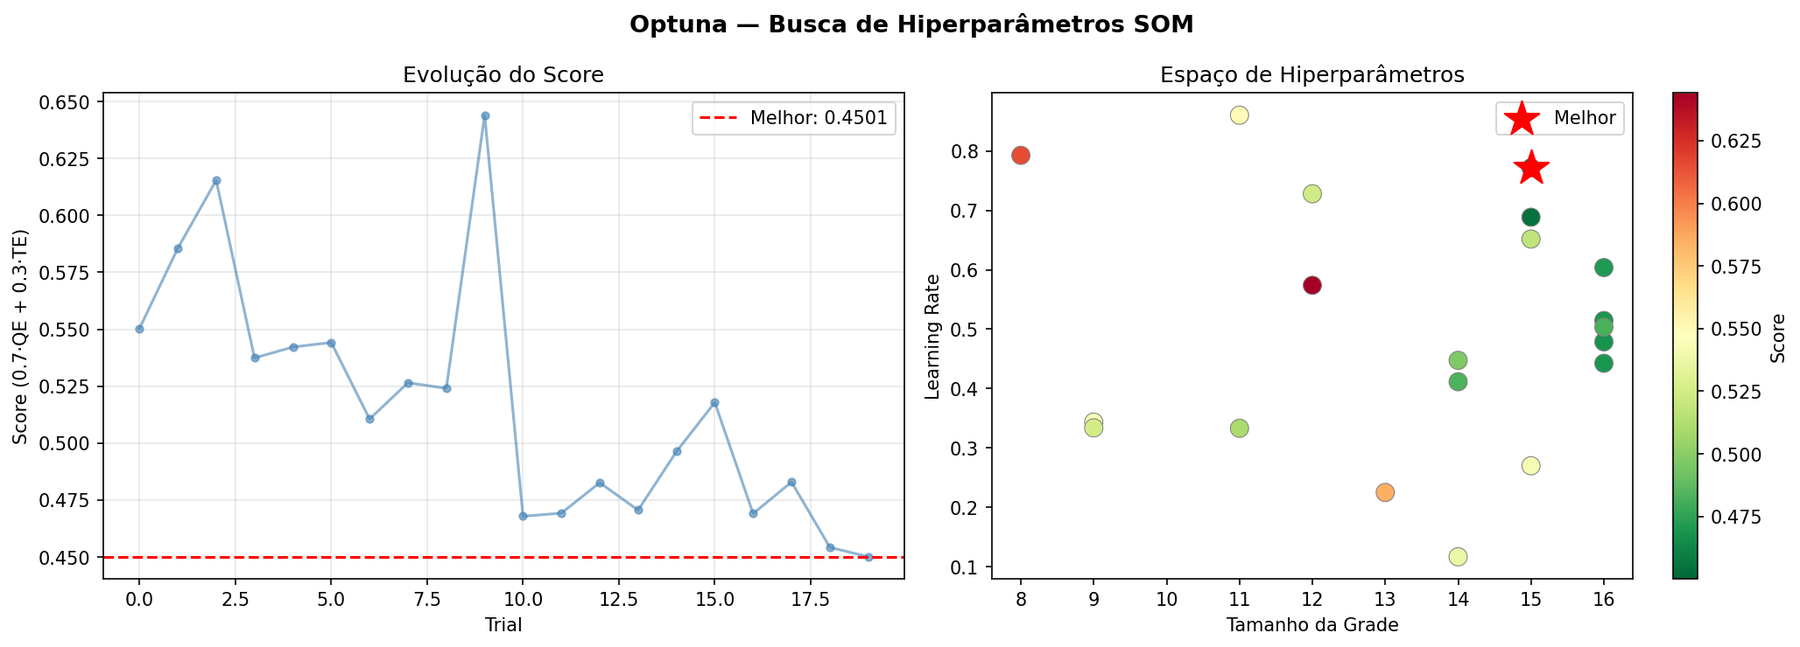
\includegraphics[width=\columnwidth]{figs/som/fig_optuna.png}
  \caption{Busca de hiperparâmetros SOM — Optuna (20~tentativas):
           evolução do score (esq.) e espaço tamanho de grade vs.\
           learning rate (dir.). Melhor configuração: $15\times15$.}
  \label{fig:som_optuna}
\end{figure}

\subsection{Resultados}

\subsubsection{Qualidade do Modelo}

\begin{table}[!t]
  \caption{Métricas de qualidade da SOM ($15\times15$ neurônios)}
  \label{tab:som_quality}
  \centering
  \begin{tabular}{lll}
    \toprule
    \textbf{Métrica} & \textbf{Valor} & \textbf{Interpretação} \\
    \midrule
    Quantization Error (QE) & 0,572
      & Bom — neurônios representam bem os pixels \\
    Topographic Error (TE)  & 0,133
      & Bom — vizinhança espacial preservada \\
    Silhouette              & 0,341
      & Aceitável — classes com alguma sobreposição \\
    \bottomrule
  \end{tabular}
\end{table}

\begin{figure}[!t]
  \centering
  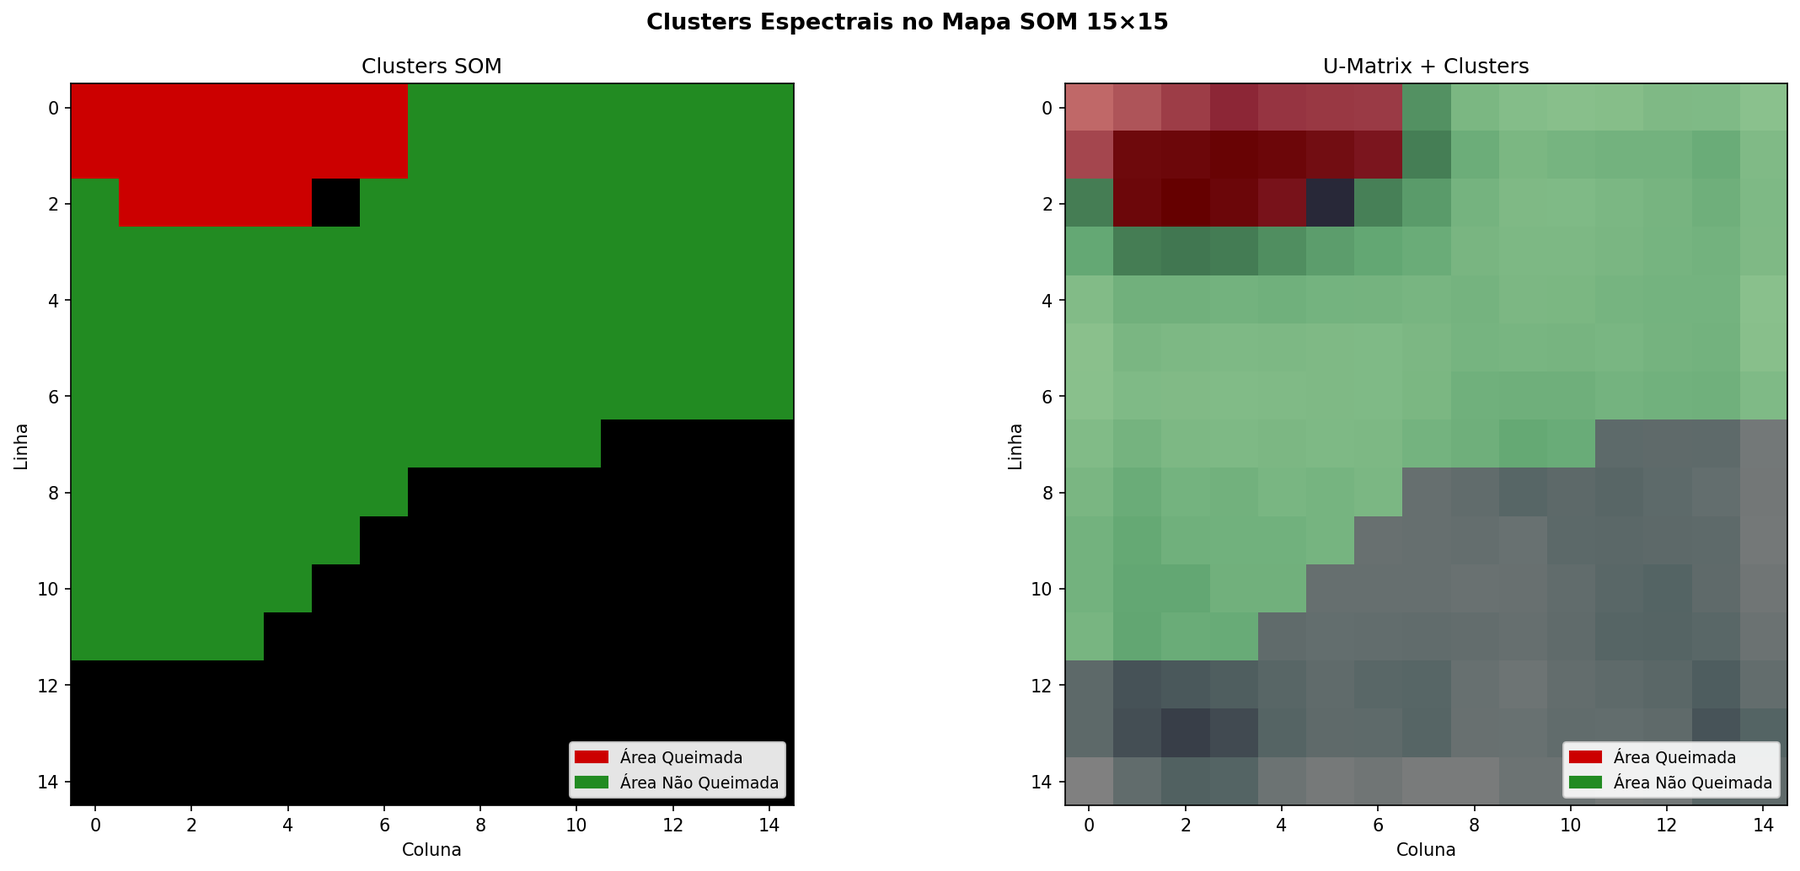
\includegraphics[width=\columnwidth]{figs/som/fig_clusters.png}
  \caption{Organização topológica da SOM $15\times15$: grade com clusters
           K-Means sobrepostos à U-Matrix (esq.) e separação inter-cluster
           com área por classe em hectares (dir.).}
  \label{fig:som_clusters}
\end{figure}

\subsubsection{Estimativa de Área Queimada}

\begin{table}[!t]
  \caption{Distribuição das classes e área estimada — Cena 221/074}
  \label{tab:som_area}
  \centering
  \begin{tabular}{lcc}
    \toprule
    \textbf{Classe} & \textbf{\% da Cena} & \textbf{Área (hectares)} \\
    \midrule
    Não Queimada & $\sim$93\%  & $\sim$3.322.000 \\
    Queimada     & $\sim$4,3\% & $\sim$154.000   \\
    Água         & $\sim$2,7\% & $\sim$97.000    \\
    \bottomrule
  \end{tabular}
\end{table}

\subsubsection{Saída Espacial}

Na composição falsa-cor B7/B5/B4, as áreas queimadas aparecem em vermelho
intenso. O mapa SOM concorda espacialmente com essas assinaturas, como
demonstra a Fig.~\ref{fig:som_mapa}.

\begin{figure}[!t]
  \centering
  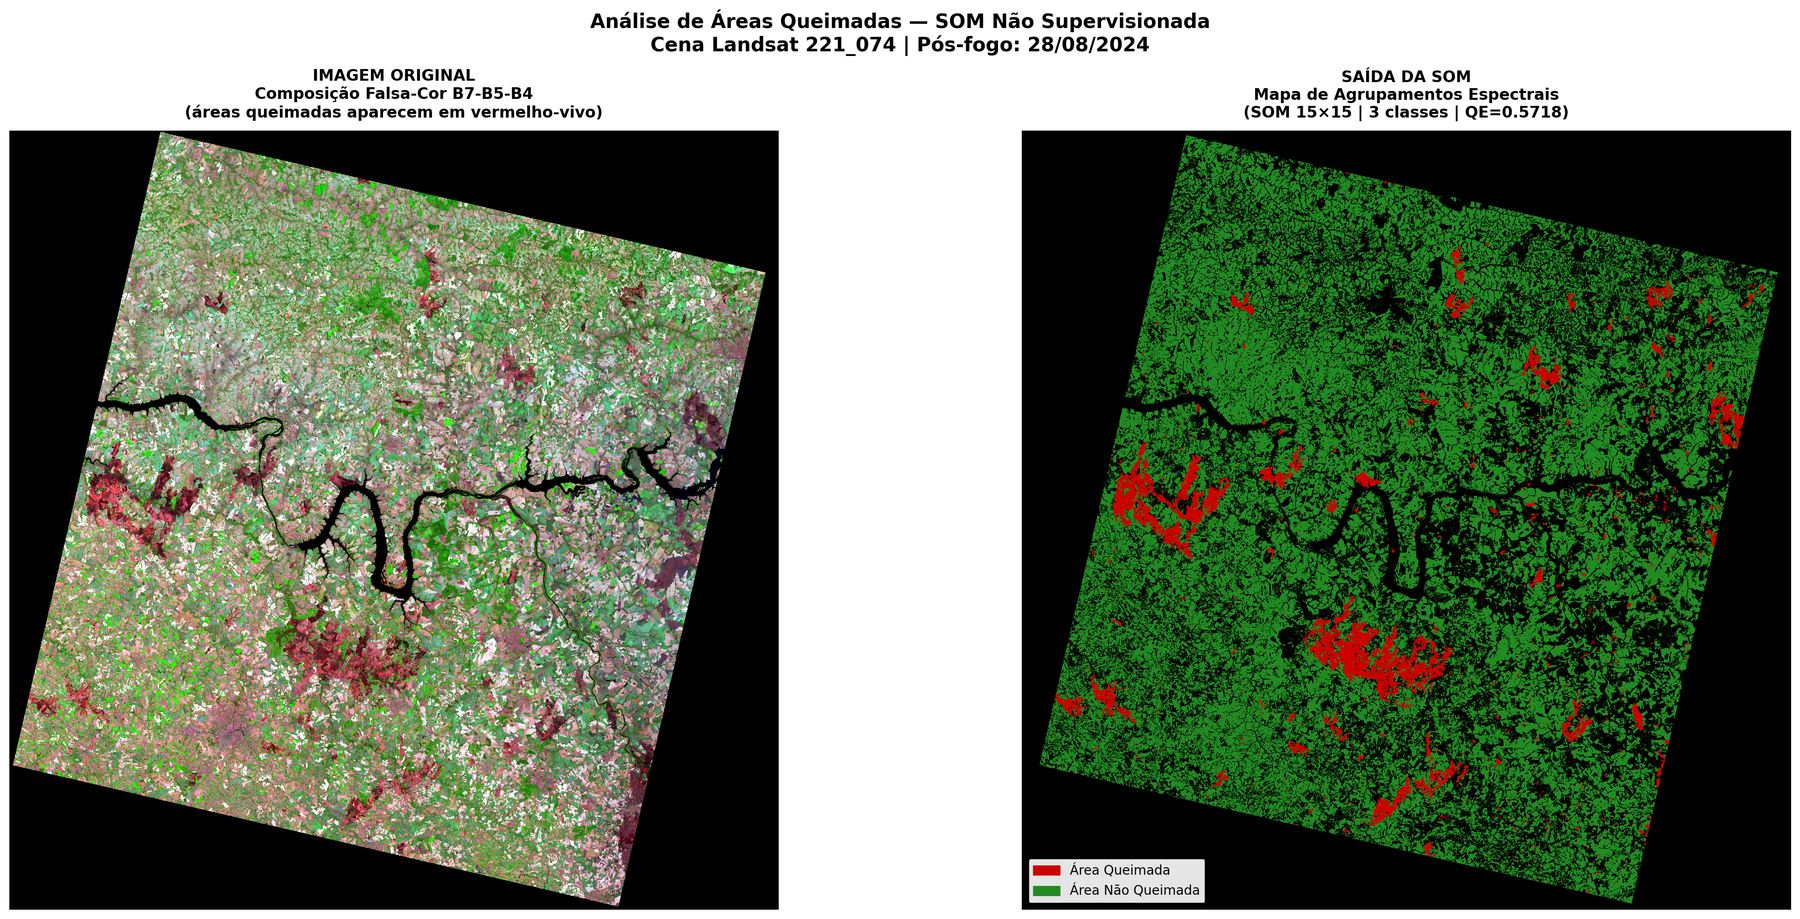
\includegraphics[width=\columnwidth]{figs/som/fig_mapa.png}
  \caption{Esquerda: composição falsa-cor pós-queimada (áreas queimadas
           em vermelho). Direita: mapa de classificação SOM ($15\times15$,
           3~classes, QE=0,572) — cicatrizes identificadas sem rótulos.}
  \label{fig:som_mapa}
\end{figure}

\subsection{Discussão}

A SOM dispensou completamente amostras rotuladas, podendo ser aplicada
a qualquer cena Landsat sem trabalho de campo — vantagem operacional
significativa em regiões de difícil acesso. A heurística de atribuição
pode falhar em regiões com solo exposto por seca severa, onde a assinatura
espectral se confunde com cicatrizes de fogo. Ao contrário de métodos
supervisionados, não é possível calcular métricas como F1 ou AUC sem
referência externa — a qualidade é avaliada por métricas internas (QE, TE,
Silhouette) e inspeção visual.

%=====================================================================
\section{Random Forest}

\subsection{Entradas, Saídas e Objetivo}

\textbf{Objetivo:} classificação binária supervisionada pixel a pixel
com validação por blocos espaciais, comparando estratégias de tratamento
de desbalanceamento e avaliando generalização entre cenas.

\subsection{Metodologia}

\subsubsection{Pipeline de Processamento}

\begin{enumerate}
  \item \textbf{Carregamento e alinhamento}: leitura das bandas GeoTIFF via
        \texttt{rasterio}, \textit{shape} mínima comum entre todos os arquivos.
  \item \textbf{Mascaramento de validade}: exclusão de pixels com
        \textit{nodata}, NaN ou rótulo fora de $\{0,1\}$.
  \item \textbf{Subamostragem estratificada}: 150.000~pixels por cena,
        preservando proporção original de classes.
  \item \textbf{Validação por blocos espaciais}: grade $4\times4$
        (16~blocos), 4~blocos ($\approx25\%$) para teste.
  \item \textbf{Tratamento de desbalanceamento}: uma das quatro estratégias.
  \item \textbf{Treinamento e otimização}: RandomizedSearchCV (30~iterações,
        5-\textit{fold} CV, critério $F_1$).
  \item \textbf{Ajuste de threshold}: otimização via curva Precision-Recall,
        maximizando $F_2$ (Eq.~\ref{eq:f2}).
  \item \textbf{Validação cruzada entre cenas}: treino em 221/074,
        teste em 220/075.
\end{enumerate}

\begin{equation}
  \tau^* = \underset{\tau}{\arg\max}\;
  F_2(\tau) = \frac{5 \cdot P(\tau) \cdot R(\tau)}
                   {4 \cdot P(\tau) + R(\tau)}
  \label{eq:f2}
\end{equation}

\subsubsection{Controle de Leakage}

Os índices \textit{dNBR} e \textit{dNDVI} foram explicitamente excluídos
do vetor de atributos. A máscara de referência foi gerada com limiar
$\mathrm{dNBR} > 0{,}65$: incluí-los como \textit{features} criaria
circularidade direta, produzindo métricas artificialmente perfeitas
($F_2 = 1{,}000$, Kappa~$= 1{,}000$).

\subsubsection{Validação por Blocos Espaciais}

Cada pixel $(r,c)$ é atribuído ao bloco
$b = \lfloor r/H \cdot k \rfloor \cdot k + \lfloor c/W \cdot k \rfloor$,
com $k=4$ e $(H,W)$ o tamanho da cena. A Fig.~\ref{fig:rf_blocos} ilustra
a divisão aplicada à cena~221/074.

\begin{figure}[!t]
  \centering
  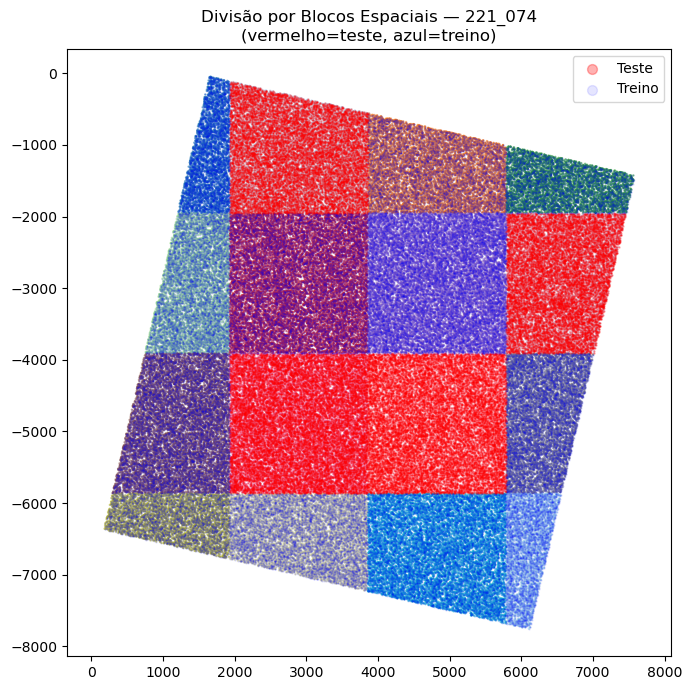
\includegraphics[width=0.85\columnwidth]{figs/rf/fig_blocos_espaciais.png}
  \caption{Divisão por blocos espaciais ($4\times4$, 16~blocos), cena 221/074.
           Vermelho = teste (blocos~1, 7, 9, 10); azul = treino.}
  \label{fig:rf_blocos}
\end{figure}

\subsection{Resultados}

\subsubsection{Comparação das Estratégias de Desbalanceamento}

\begin{table}[!t]
  \caption{Comparação de estratégias de desbalanceamento — RF, cena 221/074}
  \label{tab:rf_estrategias}
  \centering
  \setlength{\tabcolsep}{3.5pt}
  \begin{tabular}{lcccccc}
    \toprule
    \textbf{Estratégia} & \textbf{$F_2$} & \textbf{MCC} & \textbf{Kappa}
                        & \textbf{Prec.} & \textbf{Recall} & \textbf{AUPRC} \\
    \midrule
    Sem tratamento          & 0,021 & 0,088 & 0,030 & 0,535 & 0,017 & 0,202 \\
    \textit{class\_weight}  & 0,017 & 0,086 & 0,024 & 0,632 & 0,013 & 0,191 \\
    SMOTE                   & 0,234 & 0,173 & 0,172 & 0,200 & 0,245 & 0,154 \\
    SMOTETomek              & 0,235 & 0,173 & 0,172 & 0,200 & 0,245 & 0,158 \\
    Undersampling           & \textbf{0,354} & \textbf{0,198} & 0,122
                            & 0,117 & \textbf{0,716} & 0,216 \\
    \textit{class\_weight} + $\tau^*$  & 0,346 & 0,198 & 0,151 & 0,140 & 0,547 & 0,191 \\
    \bottomrule
  \end{tabular}
\end{table}

\begin{figure}[!t]
  \centering
  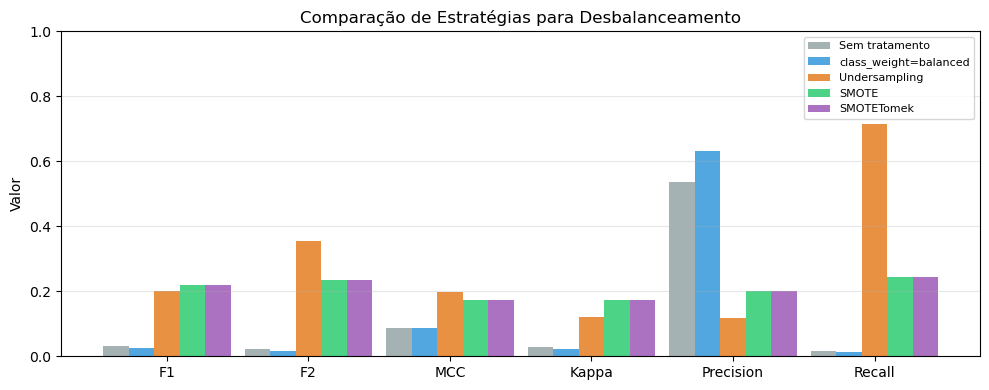
\includegraphics[width=\columnwidth]{figs/rf/fig_estrategias_comp.png}
  \caption{Comparação visual das estratégias RF por métrica ($F_2$, MCC,
           Kappa, $F_1$, Precision, Recall). Undersampling lidera em $F_2$
           e Recall com threshold padrão.}
  \label{fig:rf_estrategias}
\end{figure}

\begin{figure}[!t]
  \centering
  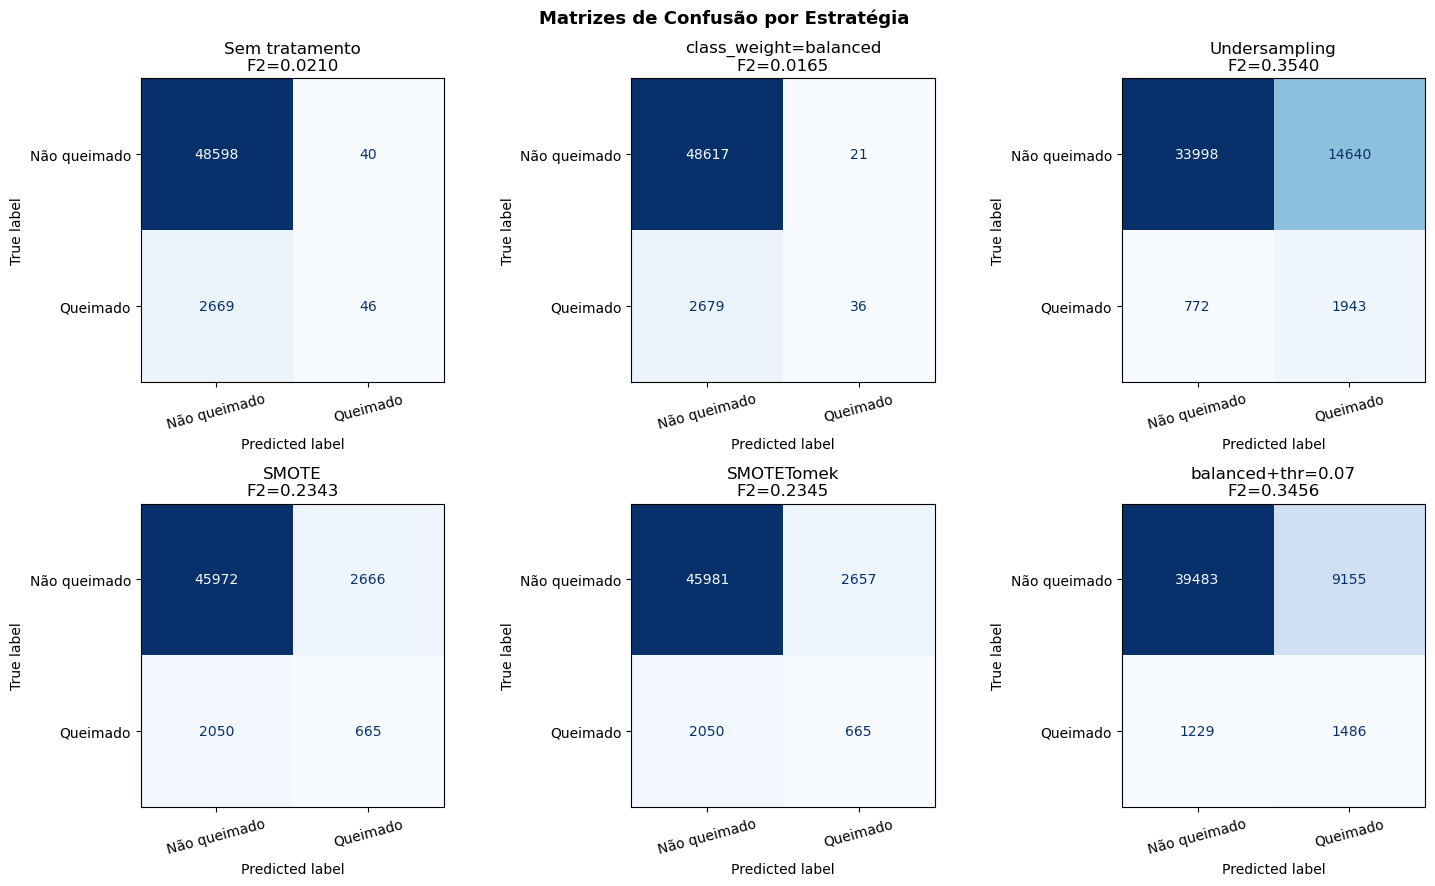
\includegraphics[width=\columnwidth]{figs/rf/fig_conf_matrices.png}
  \caption{Matrizes de confusão normalizadas para cada estratégia RF —
           cena~221/074. Undersampling maximiza o Recall (células TP mais
           escuras) ao custo de maior taxa de FP.}
  \label{fig:rf_conf_matrices}
\end{figure}

\subsubsection{Otimização de Hiperparâmetros}

O RandomizedSearchCV (30~iterações, 5-\textit{fold} CV) retornou:
\texttt{class\_weight=balanced}, \texttt{max\_depth=30},
\texttt{max\_features=sqrt}, \texttt{min\_samples\_leaf=11},
\texttt{min\_impurity\_decrease=$10^{-4}$}, \texttt{n\_estimators=171}.
Melhor $F_1$ em validação cruzada: $0{,}2211$.

\subsubsection{Modelo Otimizado e Ajuste de Threshold}

\begin{table}[!t]
  \caption{RF otimizado — efeito do ajuste de threshold}
  \label{tab:rf_otimizado}
  \centering
  \begin{tabular}{lcccccc}
    \toprule
    \textbf{Configuração} & \textbf{$F_2$} & \textbf{MCC} & \textbf{Kappa}
                          & \textbf{Prec.} & \textbf{Recall} & $\tau$ \\
    \midrule
    RF Otimizado $\tau=0{,}5$ & 0,379 & 0,267 & 0,248 & 0,224 & 0,459 & 0,50 \\
    RF Otimizado $\tau^*$     & \textbf{0,395} & 0,247 & 0,194 & 0,167 & 0,601 & 0,38 \\
    \bottomrule
  \end{tabular}
\end{table}

\begin{figure}[!t]
  \centering
  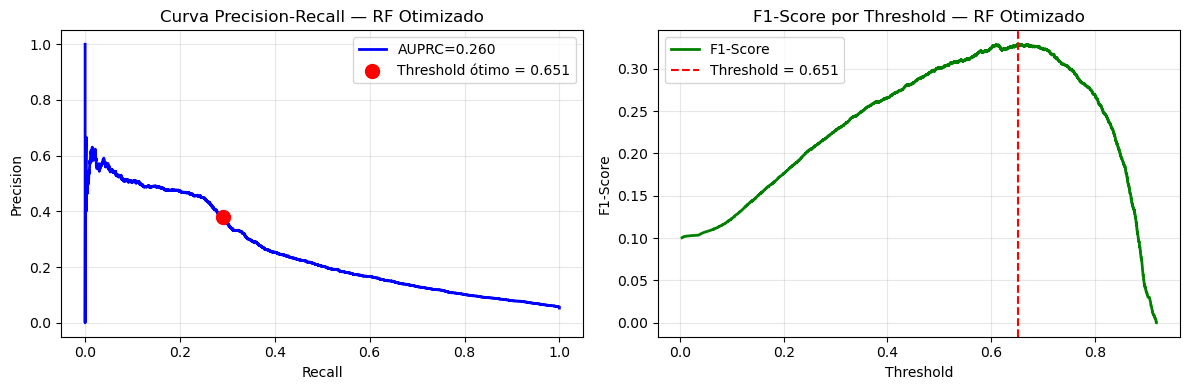
\includegraphics[width=\columnwidth]{figs/rf/fig_threshold_pr.png}
  \caption{Curva Precision-Recall e $F_2$ por threshold para o modelo
           \textit{class\_weight='balanced'}:
           $\tau^* = 0{,}07$ maximiza $F_2$ (AUPRC~$= 0{,}191$).}
  \label{fig:rf_threshold_pr}
\end{figure}

\begin{figure}[!t]
  \centering
  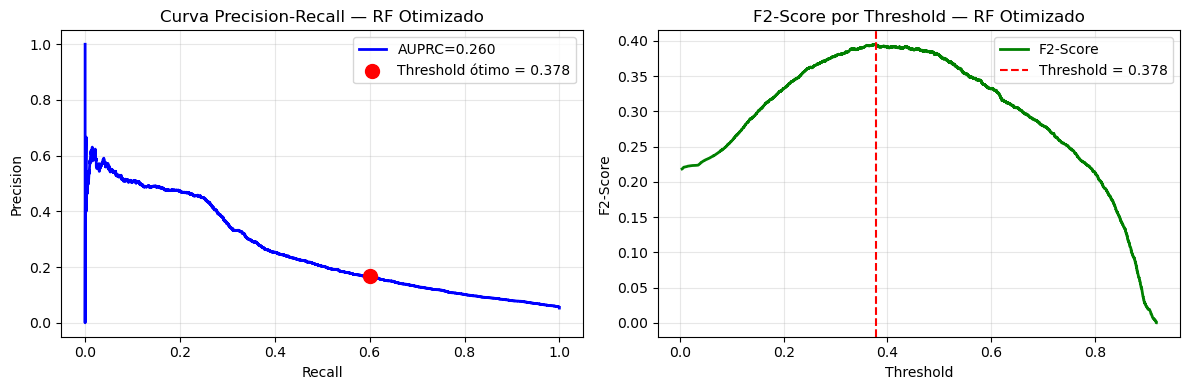
\includegraphics[width=\columnwidth]{figs/rf/fig_threshold_otimizado.png}
  \caption{RF otimizado: curva Precision-Recall com AUPRC e ponto ótimo
           (esq.); $F_2$-score por threshold com $\tau^* = 0{,}378$
           assinalado (dir.).}
  \label{fig:rf_threshold}
\end{figure}

\subsubsection{Validação Cruzada Entre Cenas}

\begin{table}[!t]
  \caption{Validação cruzada entre cenas — RF}
  \label{tab:rf_crosscena}
  \centering
  \begin{tabular}{lcccccc}
    \toprule
    \textbf{Treino $\to$ Teste} & \textbf{$F_2$} & \textbf{MCC}
    & \textbf{Kappa} & \textbf{Prec.} & \textbf{Recall} & \textbf{AUPRC} \\
    \midrule
    221/074 $\to$ Intra   & 0,395 & 0,247 & 0,194 & 0,167 & 0,601 & 0,260 \\
    221/074 $\to$ 220/075 & \textbf{0,472} & \textbf{0,292} & \textbf{0,241}
                          & 0,222 & \textbf{0,657} & \textbf{0,467} \\
    \bottomrule
  \end{tabular}
\end{table}

\subsubsection{Importância de Atributos}

\begin{table}[!t]
  \caption{Importância dos atributos — RF otimizado}
  \label{tab:rf_importancia}
  \centering
  \begin{tabular}{clc}
    \toprule
    \textbf{Rank} & \textbf{Atributo} & \textbf{Importância} \\
    \midrule
    1  & pre\_ndvi & 0,1145 (11,5\%) \\
    2  & pre\_b4   & 0,1106 (11,1\%) \\
    3  & pre\_nbr  & 0,1094 (10,9\%) \\
    4  & pos\_nbr  & 0,1091 (10,9\%) \\
    5  & pre\_b7   & 0,1061 (10,6\%) \\
    6  & pos\_b5   & 0,0985 (9,9\%)  \\
    7  & pre\_b5   & 0,0956 (9,6\%)  \\
    8  & pos\_ndvi & 0,0899 (9,0\%)  \\
    9  & pos\_b7   & 0,0835 (8,4\%)  \\
    10 & pos\_b4   & 0,0828 (8,3\%)  \\
    \bottomrule
  \end{tabular}
\end{table}

\begin{figure}[!t]
  \centering
  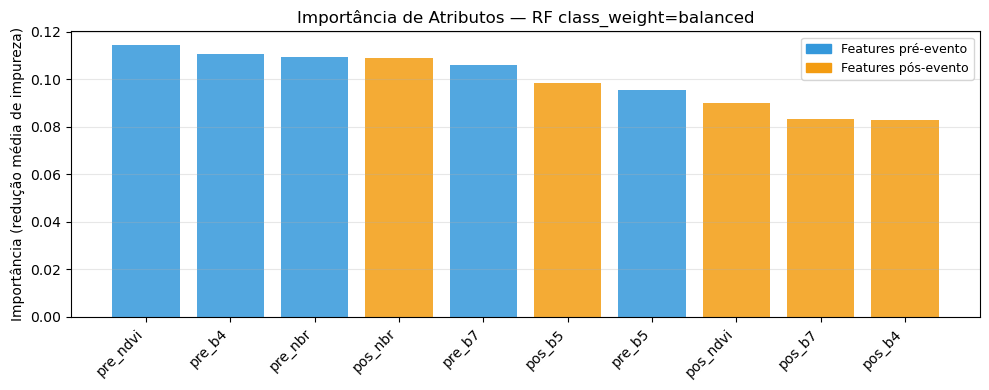
\includegraphics[width=\columnwidth]{figs/rf/fig_importancia.png}
  \caption{Importância de atributos RF (redução média de impureza Gini).
           Azul = pré-evento; laranja = pós-evento. Distribuição uniforme
           (8,3\%--11,5\%) confirma ausência de leakagem.}
  \label{fig:rf_importancia}
\end{figure}

\subsubsection{Ranking Final das Estratégias}

\begin{figure}[!t]
  \centering
  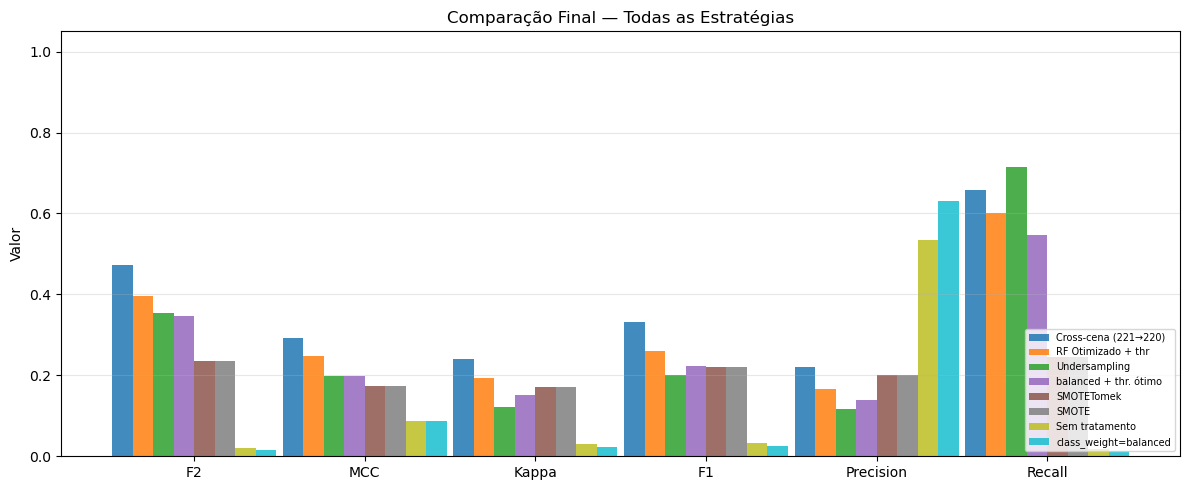
\includegraphics[width=\columnwidth]{figs/rf/fig_ranking_final.png}
  \caption{Ranking final das estratégias RF por métrica. Undersampling
           lidera em $F_2$ e Recall; \textit{class\_weight} com $\tau^*$
           equilibra melhor Precision e Kappa.}
  \label{fig:rf_ranking}
\end{figure}

\subsubsection{Mapa de Predição}

\begin{table}[!t]
  \caption{Métricas do mapa de predição completo — RF, cena 221/074}
  \label{tab:rf_mapa}
  \centering
  \begin{tabular}{lrr}
    \toprule
    \textbf{Classe predita} & \textbf{Ref.\ Queimado} & \textbf{Ref.\ Não queimado} \\
    \midrule
    Predito Queimado     & TP = 1.467 & FP = 10.307 \\
    Predito Não queimado & FN = 1.405 & TN = 47.271 \\
    \midrule
    \textbf{Precision}  & \multicolumn{2}{c}{12,46\%} \\
    \textbf{Recall}     & \multicolumn{2}{c}{51,08\%} \\
    \textbf{$F_2$}      & \multicolumn{2}{c}{0,3153}  \\
    \textbf{\% pred.\ queimado} & \multicolumn{2}{c}{19,5\% (real: 4,8\%)} \\
    \bottomrule
  \end{tabular}
\end{table}

\subsection{Discussão}

O experimento com RF demonstrou explicitamente o impacto da circularidade:
com \textit{dNBR}/\textit{dNDVI} como \textit{features}, todas as
estratégias atingiam $F_2 = 1{,}000$ e Kappa~$= 1{,}000$. Após a remoção,
os valores caíram para intervalos realistas ($F_2 \in [0{,}02,\,0{,}47]$)
e a importância distribuiu-se uniformemente. O Undersampling superou
SMOTE/SMOTETomek, possivelmente porque amostras sintéticas geradas por
interpolação em regiões de fronteira espectral degradam a fronteira de
decisão. O resultado da validação cross-cena ($F_2 = 0{,}472$) confirma
que o modelo aprende relações espectrais que transferem entre órbitas e
entre Landsat~8 e~9.

%=====================================================================
\section{Discussão Comparativa}

\subsection{Protocolo de Validação e Comparabilidade}

A Tabela~\ref{tab:comparacao_geral} consolida os resultados de todos os
modelos. As diferenças de protocolo — cenas de treino/teste, tamanho de
amostra, forma de validação — limitam a comparação direta.

\begin{table}[!t]
  \caption{Comparação geral dos modelos}
  \label{tab:comparacao_geral}
  \centering
  \setlength{\tabcolsep}{3pt}
  \begin{tabular}{llccccc}
    \toprule
    \textbf{Modelo} & \textbf{Cena Teste} & \textbf{Recall}
                    & \textbf{Prec.} & \textbf{F1} & \textbf{AUC} & \textbf{Feats.} \\
    \midrule
    KNN (interno) & intra-cena (30\%)  & 0,770 & 0,710 & 0,740 & — & 3  \\
    KNN (nova cena) & cena independente & 0,820 & 0,090 & 0,170 & — & 3  \\
    SVM Linear    & 222/074 (amostras) & 0,834 & 0,140 & 0,240 & — & 2  \\
    SVM RBF       & 221/074 (cego)     & 0,996 & 0,986 & 0,991 & 1,000 & 10 \\
    SVM RBF       & 222/074 (cego)     & 0,993 & 0,968 & 0,981 & 1,000 & 10 \\
    MLP (CV)      & 220/075+221/074    & 0,693 & 0,753 & 0,722 & 0,812 & 10 \\
    MLP (cego)    & 222/074 (40M)      & 0,713 & 0,116 & 0,199 & 0,830 & 10 \\
    SOM$^{*}$     & 221/074            & —     & —     & —     & —     & 7  \\
    RF (blocos)   & 221/074            & 0,601 & 0,167 & — & — ($F_2$=0,395) & 10 \\
    RF (cross)    & 220/075            & 0,657 & 0,222 & — & — ($F_2$=0,472) & 10 \\
    \bottomrule
    \multicolumn{7}{l}{$^{*}$SOM: QE=0,572, TE=0,133, Silhouette=0,341.}
  \end{tabular}
\end{table}

A disparidade entre SVM~RBF ($F_1 > 98\%$) e demais modelos é parcialmente
explicada por protocolo: a SVM~RBF foi validada em toda a imagem cega,
enquanto o RF usou validação por blocos espaciais — o protocolo mais
conservador. O MLP ilustra claramente o efeito do desbalanceamento:
AUC~$= 0{,}830$ indica boa separabilidade, mas a Precision de 11,6\% com
threshold~0,5 revela o impacto de treinar com 50/50 e testar em 97:3.

\subsection{Papel dos Atributos}

A comparação entre SVM~Linear (2~atributos, $F_1 = 24\%$) e SVM~RBF
(10~atributos, $F_1 > 98\%$) evidencia o ganho ao incorporar bandas
espectrais brutas e NBR. A importância uniforme no RF (8,3\%--11,5\%)
confirma que todos os 10~atributos contribuem: nenhum domina, e atributos
pré-evento lideram marginalmente, sugerindo que o estado da vegetação
antes do incêndio é mais discriminativo.

\subsection{Leakage e Validade Metodológica}

O risco de circularidade entre atributos e rótulos é um alerta recorrente
em estudos de mapeamento remoto. Utilizar como feature o mesmo índice que
gerou a máscara é um erro silencioso: as métricas chegam a valores
perfeitos sem que nenhuma etapa da pipeline sinalize problema. A análise
de importância de atributos é a principal ferramenta de diagnóstico.

\subsection{Modelo Não Supervisionado}

A SOM oferece uma alternativa viável quando rótulos não estão disponíveis.
Detectou $\approx154$~mil hectares sem nenhuma amostra rotulada, com
resultado espacialmente coerente. Como trabalho futuro, propõe-se comparação
das saídas SOM com máscaras de referência independentes para quantificar
a acurácia espacial.

%=====================================================================
\section{Conclusão}

Este trabalho apresentou, comparou e discutiu seis abordagens de
classificação para detecção de área queimada em imagens Landsat~8/9,
enfatizando os aspectos metodológicos que condicionam a validade dos
resultados. Os principais achados são:

\begin{enumerate}
  \item O \textbf{KNN} ($K=5$) atingiu 73\% de acurácia na cena de
        treinamento, mas apresentou forte degradação ao generalizar para
        nova cena (Precision~$= 9\%$, F1~$= 0{,}17$), evidenciando baixa
        robustez espacial e sensibilidade às diferenças radiométricas
        entre cenas.
  \item A \textbf{SVM~RBF} atingiu desempenho superior nos testes cegos
        ($F_1 > 98\%$, AUC-ROC~$= 1{,}000$), demonstrando que 10~atributos
        espectrais multitemporais com kernel não-linear são altamente
        discriminativos.
  \item O \textbf{RF com validação por blocos espaciais} forneceu a
        avaliação mais conservadora e metodologicamente rigorosa:
        $F_2 = 0{,}472$ em generalização cross-cena, com distribuição
        uniforme de importância confirmando ausência de leakagem.
  \item A \textbf{MLP} apresentou AUC~$= 0{,}830$ no teste cego, mas
        métricas de classificação degradadas pelo desbalanceamento —
        indicando a necessidade de ajuste de threshold para aplicações reais.
  \item A \textbf{SOM} detectou $\approx154$~mil hectares sem nenhum
        rótulo, sendo adequada como ferramenta de triagem e análise
        exploratória.
  \item A \textbf{SVM~Linear} com apenas NDVI pré/pós mostrou Recall~$= 83\%$,
        mas baixa Precision — reforçando que atributos espectrais adicionais
        são essenciais.
  \item O controle de \textbf{leakage circular} é crítico: incluir o dNBR
        como feature (derivado da mesma máscara) inflou artificialmente todas
        as métricas para valores perfeitos.
\end{enumerate}

Como trabalhos futuros: (i)~padronizar o protocolo de validação para
permitir comparação justa entre modelos; (ii)~incorporar
\textit{dNBR}/\textit{dNDVI} com máscara de referência independente
(MapBiomas~\cite{b6}); (iii)~estender a avaliação para múltiplas cenas,
anos e biomas; (iv)~avaliar modelos baseados em gradiente (XGBoost,
LightGBM) sobre os mesmos atributos.

%=====================================================================
\begin{thebibliography}{00}

\bibitem{b1}
P.~M.~Brando, J.~K.~Balch, D.~C.~Nepstad \textit{et al.},
``Abrupt increases in Amazonian tree mortality due to drought–fire
interactions,''
\textit{Proc. Natl. Acad. Sci.}, vol.~111, no.~17, pp.~6347--6352, 2014.

\bibitem{b2}
C.~H.~Key e N.~C.~Benson,
``Landscape Assessment: Composite Burn Index,''
in \textit{FIREMON: Fire Effects Monitoring and Inventory System},
USDA Forest Service, RMRS-GTR-164-CD, 2006.

\bibitem{b3}
L.~Breiman,
``Random Forests,''
\textit{Machine Learning}, vol.~45, no.~1, pp.~5--32, Oct.\ 2001.

\bibitem{b4}
H.~Karasiak, J.-F.~Dejoux, C.~Monteil e D.~Sheeren,
``Spatial dependence between training and test sets: another pitfall of
classification accuracy assessment in remote sensing,''
\textit{Machine Learning}, vol.~111, pp.~2715--2740, 2022.

\bibitem{b5}
N.~V.~Chawla, K.~W.~Bowyer, L.~O.~Hall e W.~P.~Kegelmeyer,
``SMOTE: Synthetic Minority Over-sampling Technique,''
\textit{J. Artificial Intelligence Research}, vol.~16,
pp.~321--357, 2002.

\bibitem{b6}
MapBiomas Project,
``MapBiomas Annual Mapping of Land Use and Land Cover in Brazil,''
\texttt{https://mapbiomas.org}, 2024.

\bibitem{b7}
C.~Cortes e V.~Vapnik,
``Support-vector networks,''
\textit{Machine Learning}, vol.~20, pp.~273--297, 1995.

\bibitem{b8}
T.~Kohonen,
``Self-organized formation of topologically correct feature maps,''
\textit{Biological Cybernetics}, vol.~43, pp.~59--69, 1982.

\bibitem{b9}
J.~Vesanto e E.~Alhoniemi,
``Clustering of the self-organizing map,''
\textit{IEEE Trans. Neural Networks}, vol.~11, pp.~586--600, 2000.

\bibitem{b10}
J.~Bergstra \textit{et al.},
``Algorithms for hyper-parameter optimization,''
in \textit{Advances in Neural Information Processing Systems (NeurIPS)},
vol.~24, pp.~2546--2554, 2011.

\bibitem{b11}
Y.~LeCun, Y.~Bengio e G.~Hinton,
``Deep learning,''
\textit{Nature}, vol.~521, pp.~436--444, 2015.

\bibitem{b12}
F.~Pedregosa \textit{et al.},
``Scikit-learn: Machine Learning in Python,''
\textit{J. Machine Learning Research}, vol.~12, pp.~2825--2830, 2011.

\bibitem{b13}
E.~Chuvieco \textit{et al.},
``Generation and analysis of a new global burned area product based on
MODIS 250~m reflectance bands,''
\textit{Earth System Science Data}, vol.~11, pp.~529--551, 2019.

\end{thebibliography}

\end{document}
